% ASSIGNMENT 2 LINEAR STOCHASTIC MODELLING

\section{Linear Stochastic Modelling}

% 2.1 ACF of uncorrelated and correlated sequences
\subsection{ACF of uncorrelated and correlated sequences}

\lhead{Advanced Signal Processing}
\rhead{Linear Stochastic Modelling}

\subsubsection{Using MATLAB \textbf{\code{xcorr()}} function}

Using the \code{randn()} function in MATLAB, a 1000-sample WGN process was generated, and then its ACF was estimated using the \code{xcorr()} function. The result is displayed in Figure \ref{fig:acf_est}.

\begin{figure}[H]
    \centering
    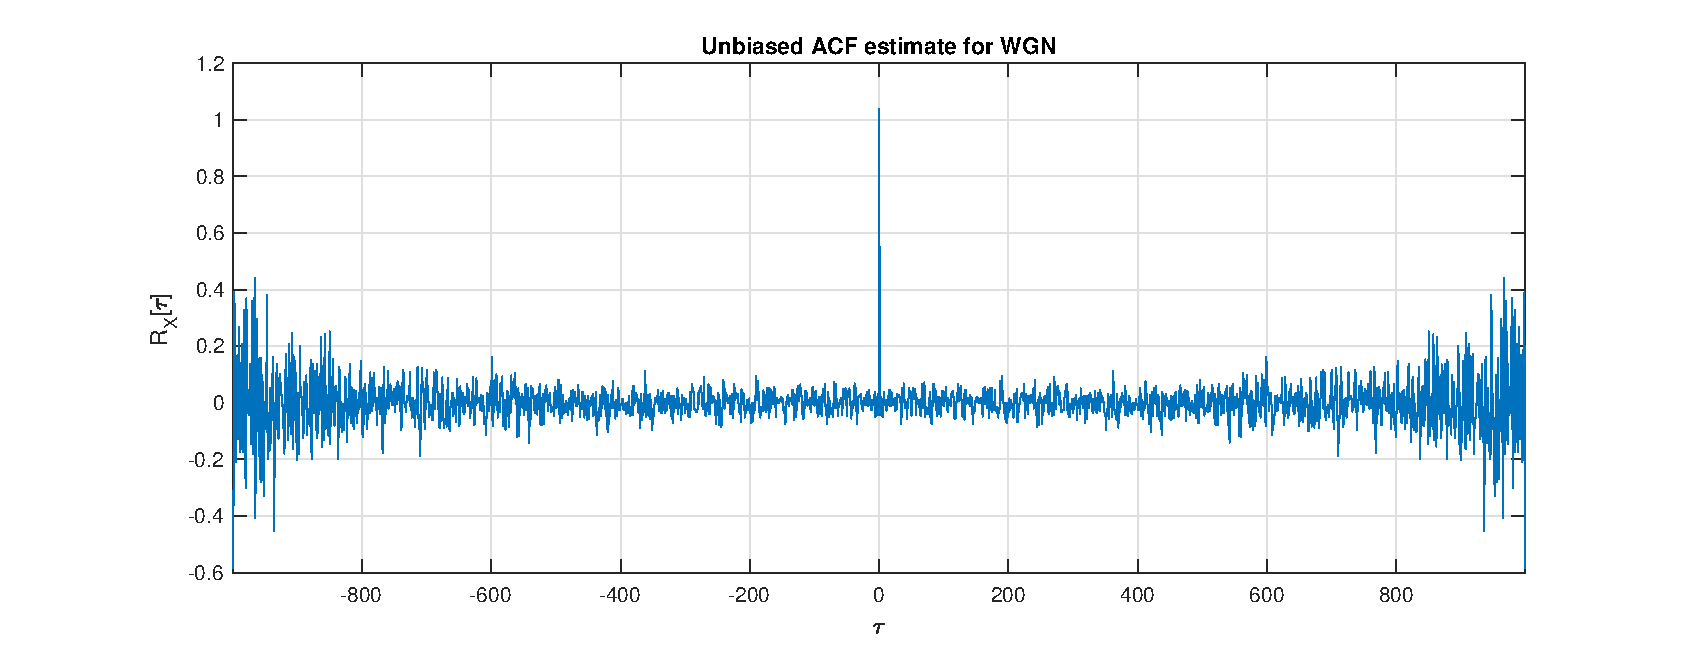
\includegraphics[width=14cm]{assignment2figs/acfest.eps}
    \caption{Unbiased estimate of ACF of 1000-sample WGN  process.}
    \label{fig:acf_est}
\end{figure}

\noindent
The ACF estimate is notably symmetric about $\tau=0$. The true ACF of a WGN process would be a Dirac delta function at $\tau=0$ and zero for all other $\tau=0$. Here, there is indeed a a Dirac delta function at $\tau=0$ but the signal is clearly not zero elsewhere. The ACF remains close to zero for $0<|\tau|<500$, but increases for $500<|\tau|<1000$. This can be explained by the fact that the number of samples included in the ACF calculation for comparison decreases (less than half of the signal is compared with itself), therefore the likelihood that the signal is self-similar increases as $|\tau| \rightarrow 1000$.

\subsubsection{ACF for small lag $\tau$}

Using MATLAB's \code{zoom()} function to focus in on $|\tau|<50$, I obtained the plot in Figure \ref{fig:acf_zoom}.

\begin{figure}[H]
    \centering
    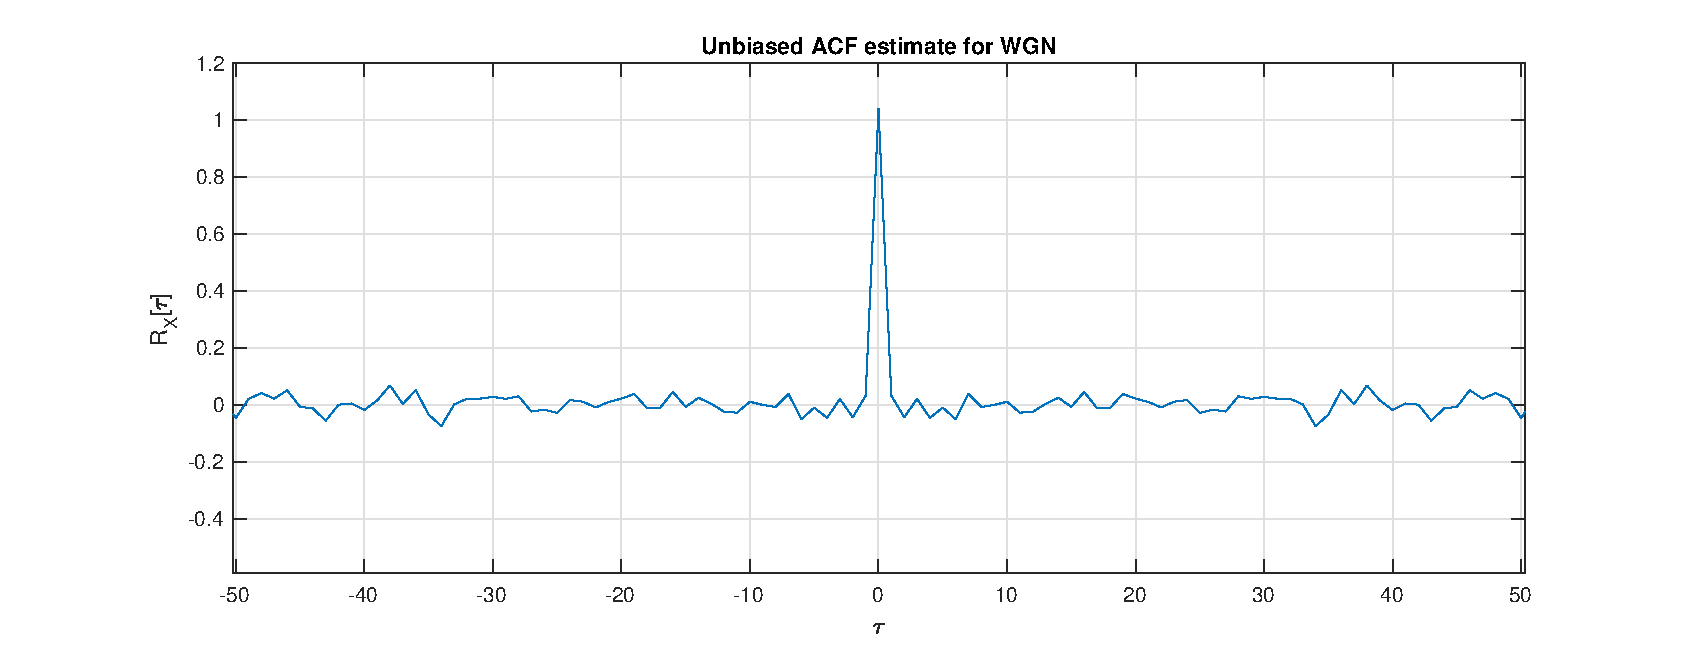
\includegraphics[width=14cm]{assignment2figs/acfzoom.eps}
    \caption{Estimate of ACF of 1000-sample WGN process.}
    \label{fig:acf_zoom}
\end{figure}

\noindent
Zooming in for small $\tau$, it is clear that the ACF estimate is a very good approximation to the ideal ACF, verifying the trend identified in the previous section.

\subsubsection{ACF for large lag $\tau$}

The unbiased ACF estimate is given by Equation \ref{eqn:unb_acf}.

\begin{equation}
\widehat{R}_{X}(\tau)=\frac{1}{N-|\tau|} \sum_{n=0}^{N-|\tau|-1} x[n] x[n+\tau], \quad \tau=-N+1, \ldots, N-1
\label{eqn:unb_acf}
\end{equation}

\noindent
It is evident from this equation that the ACF estimate $\widehat{R}_{X}(\tau)$ increases with increasing $|\tau|$ since fewer samples are included in the calculation for comparison. An empirical bound at which ACF estimates are statistically reliable would be $|\tau| < 500$. Generalising this, the bound would be  $|\tau| < \frac{N}{4}$ (where N is the number of samples in the ACF, not the original signal).

\subsubsection{Applying MA filter}

The 1000-sample WGN signal was passed through a 9th order MA filter, as well as a 5th order MA filter for comparison. The ACFs of the resultant signals are shown in Figure \ref{fig:triang}.

\begin{figure}[H]
    \centering
    \subfloat[9th order]{{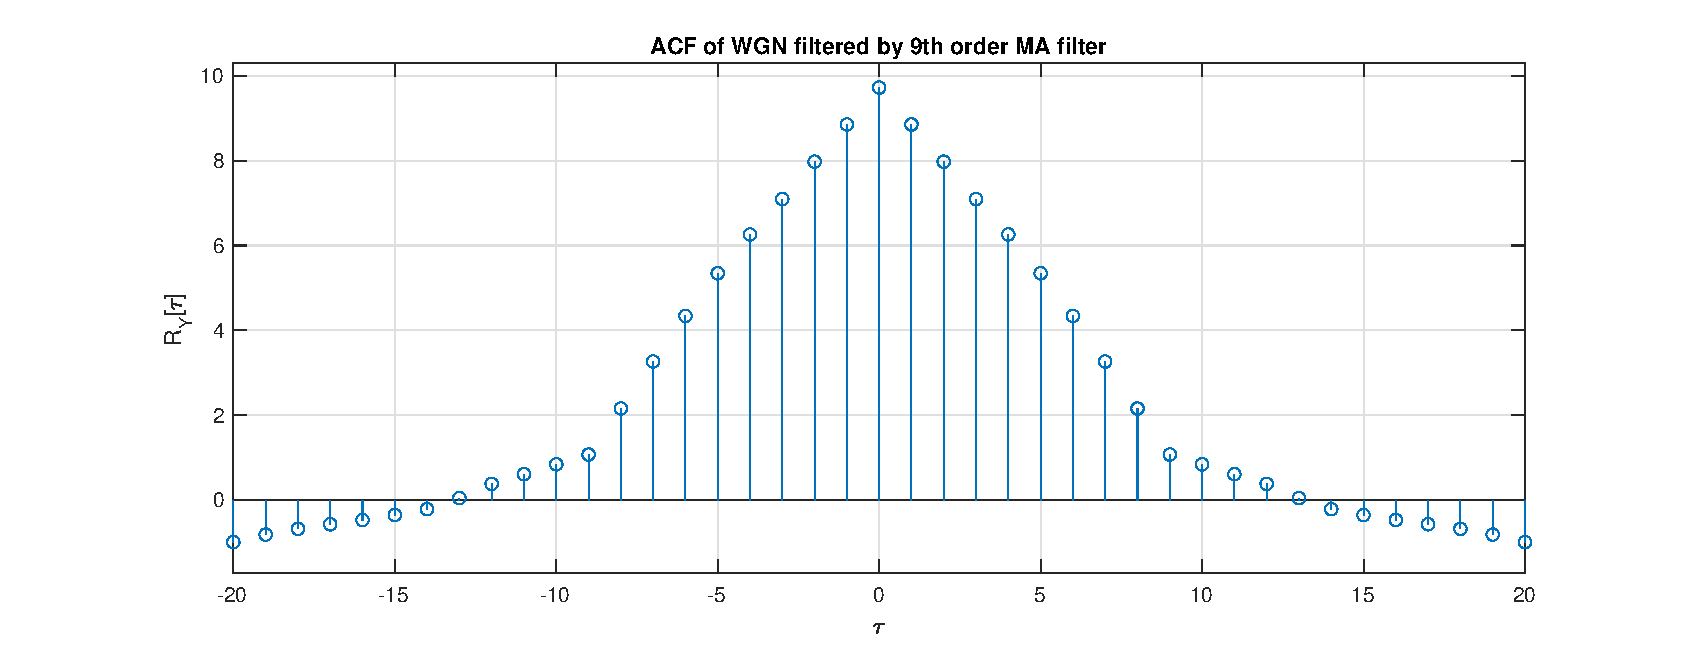
\includegraphics[width=9cm]{assignment2figs/acf_ma9.eps}}}
    \subfloat[5th order]{{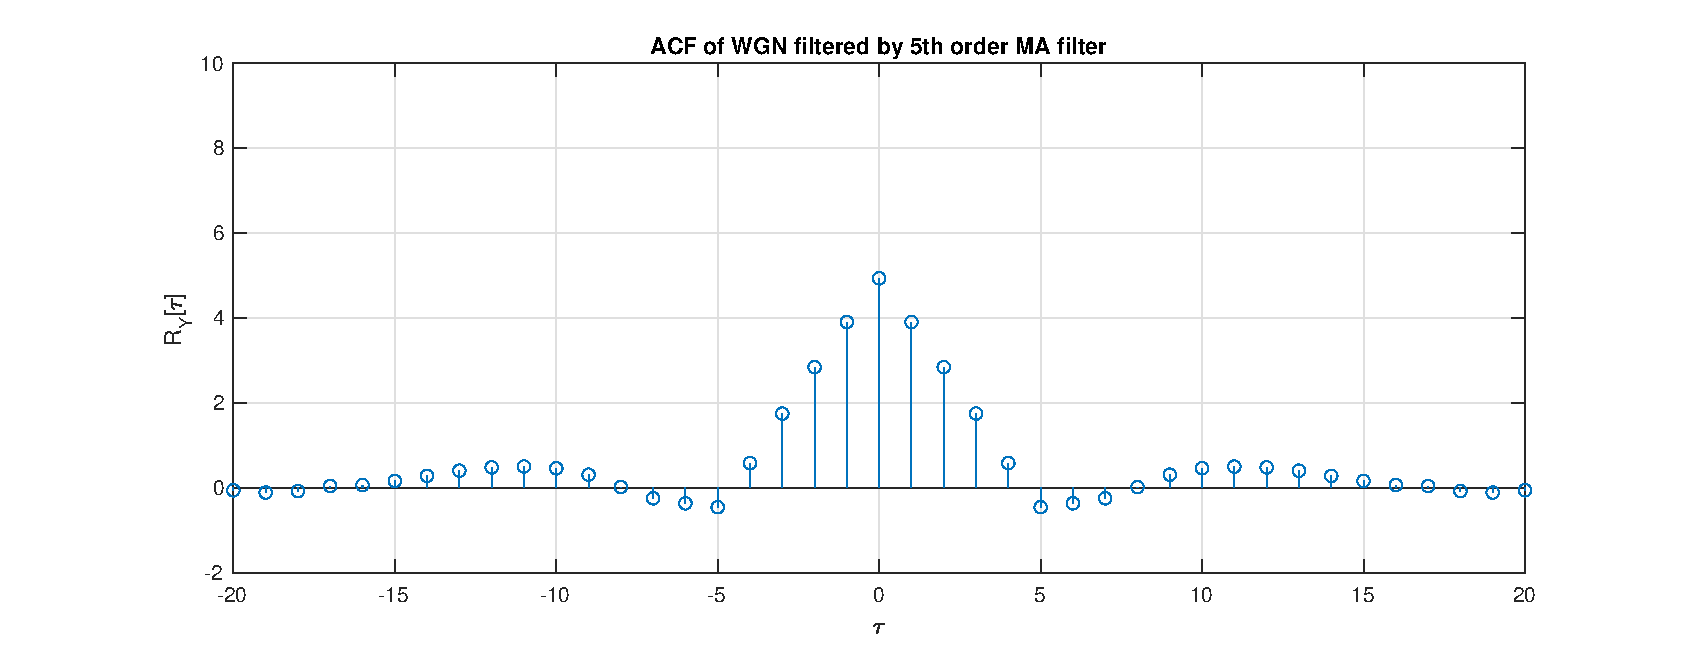
\includegraphics[width=9cm]{assignment2figs/acf_ma5.eps}}}
    \caption{ACFs of MA-filtered 1000-sample WGN process.}
    \label{fig:triang}
\end{figure}

\noindent
The ideal ACF of a MA-filtered process is $R_{T}(\tau) = N-|\tau|$ for $|\tau| < N$ and $R_{T}(\tau) =0$ otherwise (in other words, a triangular function. Figure \ref{fig:triang}(a) is indeed a triangular function with height  $\approx$ 9 and width $\approx$ 18, but we see non-zero values for $|\tau|>9$. This is because an estimate of the ACF is being used, resulting in some error. Reducing the order of the MA filter to 5, as in \ref{fig:triang}(b), the signal clearly has more oscillation as $|\tau|$ increases. This can be explained by the way a MA filter works, defined by Equation \ref{eqn:MA}.

\begin{equation}
y[n]=\sum_{i=0}^{9} b_{i} x[n-i]
\label{eqn:MA}
\end{equation}

\noindent
It works by taking the mean of the 9 previous samples and assigning this value to the current index, then shifting to the next index and repeating for all values. Through this process, an MA filter has a smoothing effect, essentially acting as a LPF. As the filter order is decreased, fewer samples are included in the averaging and therefore the signal is smoothed to a lesser extent.

\subsubsection{Uncorrelated stochastic processes}

It is given that \textbf{y} is a realisation of the stochastic process $Y_{n}$ (a filtered version of the uncorrelated process $X_{n}$) whose ACF $R_{Y}(\tau)$ is given by Equation \ref{eqn:acf_y}.

\begin{equation}
R_{Y}(\tau)=R_{X} \tau * R_{h}(\tau)
\label{eqn:acf_y}
\end{equation}

\noindent
Since $X_{n}$ is uncorrelated, its ACF $R_{X}$ must be an arbitrarily scaled Dirac delta-function $\alpha \delta(\tau)$ centered on zero. By the identity property of convolution, convolving a signal with a delta-function does not change the signal, therefore $R_{Y}(\tau) = \alpha R_{h}(\tau)$.

% 2.2 Cross-correlation function
\subsection{Cross-correlation function}

Similarly to ACF (Equation \ref{fig:acf_est}), the unbiased estimate of the CCF between two signals is given by Equation \ref{eqn:ccf}. 
\begin{equation}
\hat{R}_{X Y}(\tau)=\frac{1}{N-|\tau|} \sum_{n=0}^{N-|\tau|-1} x[n] y[n+\tau], \quad \tau=-N+1, \ldots, N-1
\label{eqn:ccf}
\end{equation}

\noindent
The CCF was calculated for the 1000-sample WGN process used in the previous section and the 9th order MA-filtered version. The result is shown in Figure \ref{fig:ccf}.

\begin{figure}[H]
    \centering
    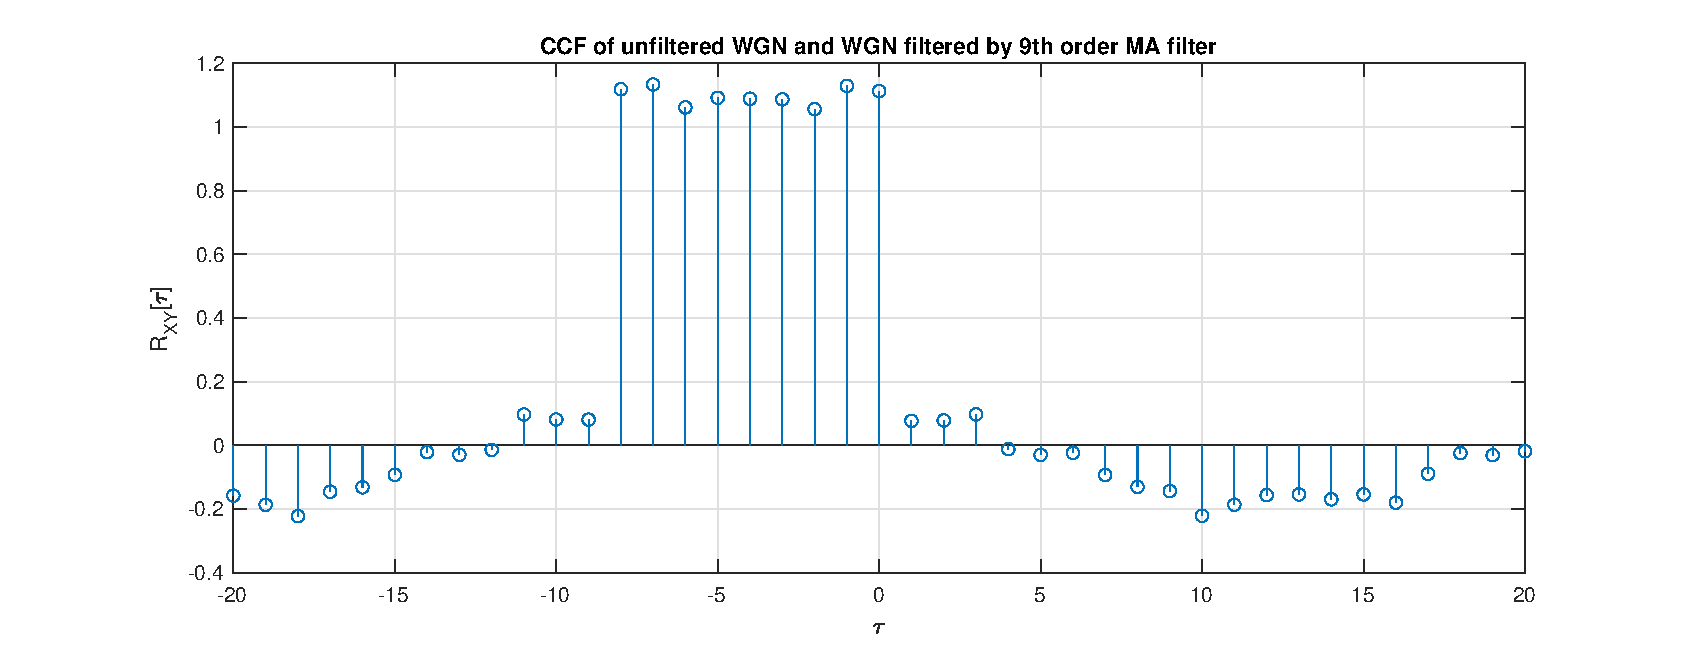
\includegraphics[width=12cm]{assignment2figs/ccf.eps}
    \caption{Estimate of CCF of 1000-sample WGN process and MA-filtered version.}
    \label{fig:ccf}
\end{figure}

\noindent
Following from the result found in the previous section, the CCF is simply the impulse response of a 9th order MA filter, which is a train of 8 delta-functions.

\subsubsection{Application to System Identification}

Generalising the relationship found in the previous section, if an uncorrelated signal is passed through an LTI system and the CCF is taken between input and outputs, the result will simply be the impulse response of the system. This is because the output of an LTI system can be found by convolving the ACF of an input with the ACF of its impulse response. If the input is simply a Dirac-delta function, the result will be the system impulse response. From LTI systems theory, it is known that the impulse response of an LTI system provides a complete characterisation of it, therefore the system can be identified.

% 2.3 Autoregressive modelling
\subsection{Autoregressive modelling}

An AR process model of order 2, denoted by AR(2), is defined by Equation \ref{eqn:ar_mod}.

\begin{equation}
x[n]=a_{1} x[n-1]+a_{2} x[n-2]+w[n], \text { where } w[n] \sim N(0,1)
\label{eqn:ar_mod}
\end{equation}

\noindent
The coefficients $a_{1} \in [-2.5,2.5] ,a_{2} \in [-1.5,1.5]$ determine the stability of the model. The region of convergence of $a_{1}$ and $a_{2}$  (in which the model is WSS) forms a triangle known at the 'stability triangle'. This is evident in Figure X, in which values of $a_{1}$ and $a_{2}$ for which the system is stable have been marked with an asterisk *.

\begin{figure}[H]
    \centering
    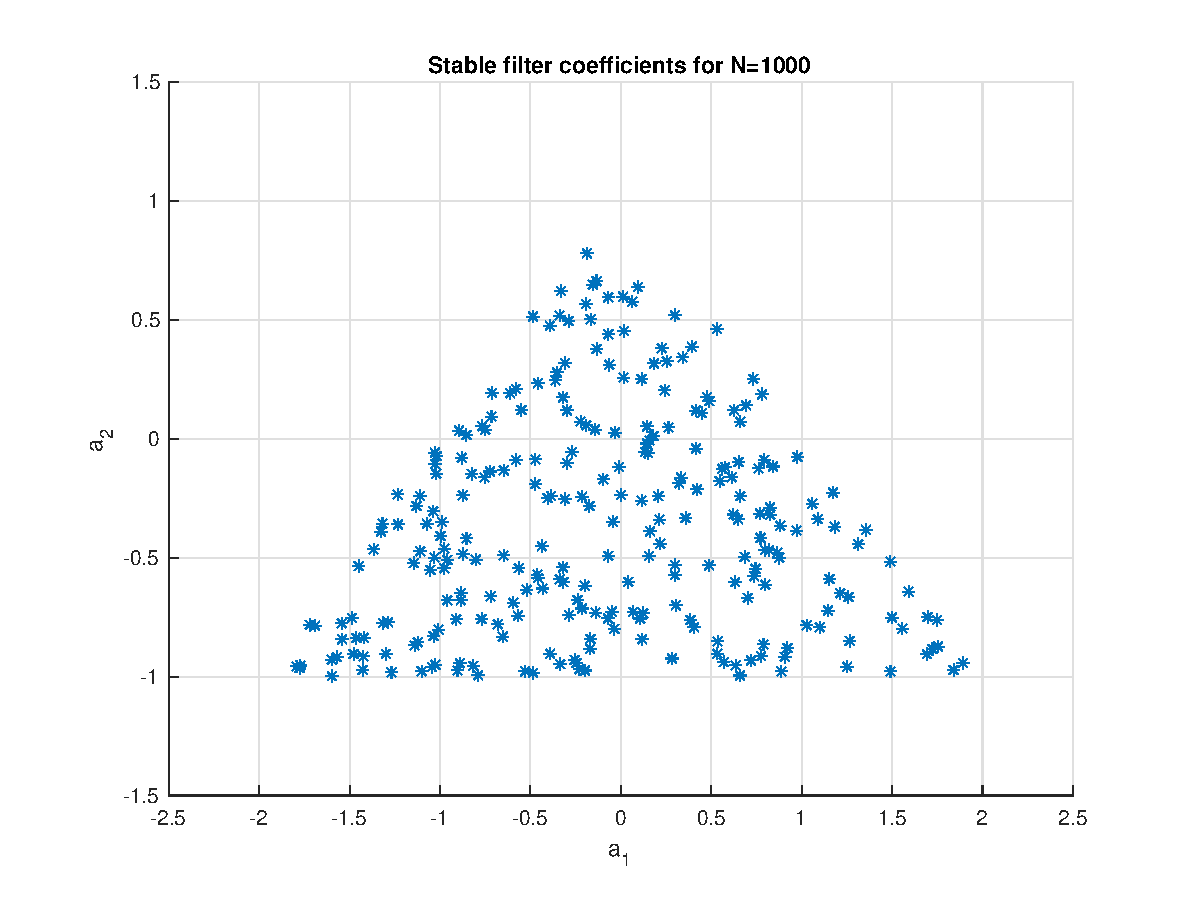
\includegraphics[width=8cm]{assignment2figs/stablecoeffs.eps}
    \caption{Stable coefficients for AR(2) process defined in Equation \ref{eqn:ar_mod}.}
    \label{fig:triangle}
\end{figure}

\noindent
This triangular shape can be explained by the fact that the system poles must lie within the unit circle for stability. The characteristic equation of the system is given by Equation \ref{eqn:char}.
\begin{equation}
C(z)=z^{2}-a_{1} z-a_{2}
\label{eqn:char}
\end{equation}
\noindent
Therefore, the system poles are given by Equation \ref{eqn:syspol}.
\begin{equation}
z=\frac{a_{1} \pm \sqrt{a_{1}^{2}+4 a_{2}}}{2}
\label{eqn:syspol}
\end{equation}

\noindent
Applying the condition that the system poles must be less than zero for stability, we obtain Equations \ref{eqn:pol1}-\ref{eqn:pol3}, which define the triangle seen in Figure \ref{fig:triangle}.

\begin{equation}
a_{1}+a_{2}<1
\label{eqn:pol1}
\end{equation}
\begin{equation}
a_{1}-a_{2}<1
\label{eqn:pol2}
\end{equation}
\begin{equation}
\left|a_{2}\right|<1
\label{eqn:pol3}
\end{equation}

\subsubsection{Sunspot Time Series}

The Sunspot time series is a dataset that has been recorded for over 300 years which indexes the number of sunspots (Wolf number) observed every year. This was loaded from MATLAB and the raw data is shown in Figure \ref{fig:sunspot}

\begin{figure}[H]
    \centering
    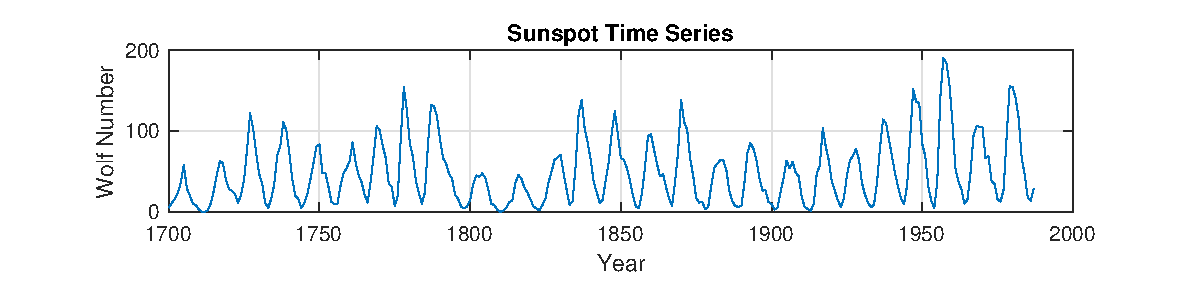
\includegraphics[width=16cm]{assignment2figs/sunspot.eps}
    \caption{Raw Sunspot Time Series data.}
    \label{fig:sunspot}
\end{figure}

\noindent
The ACFs of the Sunspot data were calculated for both the raw Sunspot data and the standardised Sunspot data for data lengths N = 5, N = 20 and N = 250. These are shown in Figure \ref{fig:sun_acfs}.

\begin{figure}[H]
    \begin{center}
\begin{subfigure}{0.5\textwidth}
  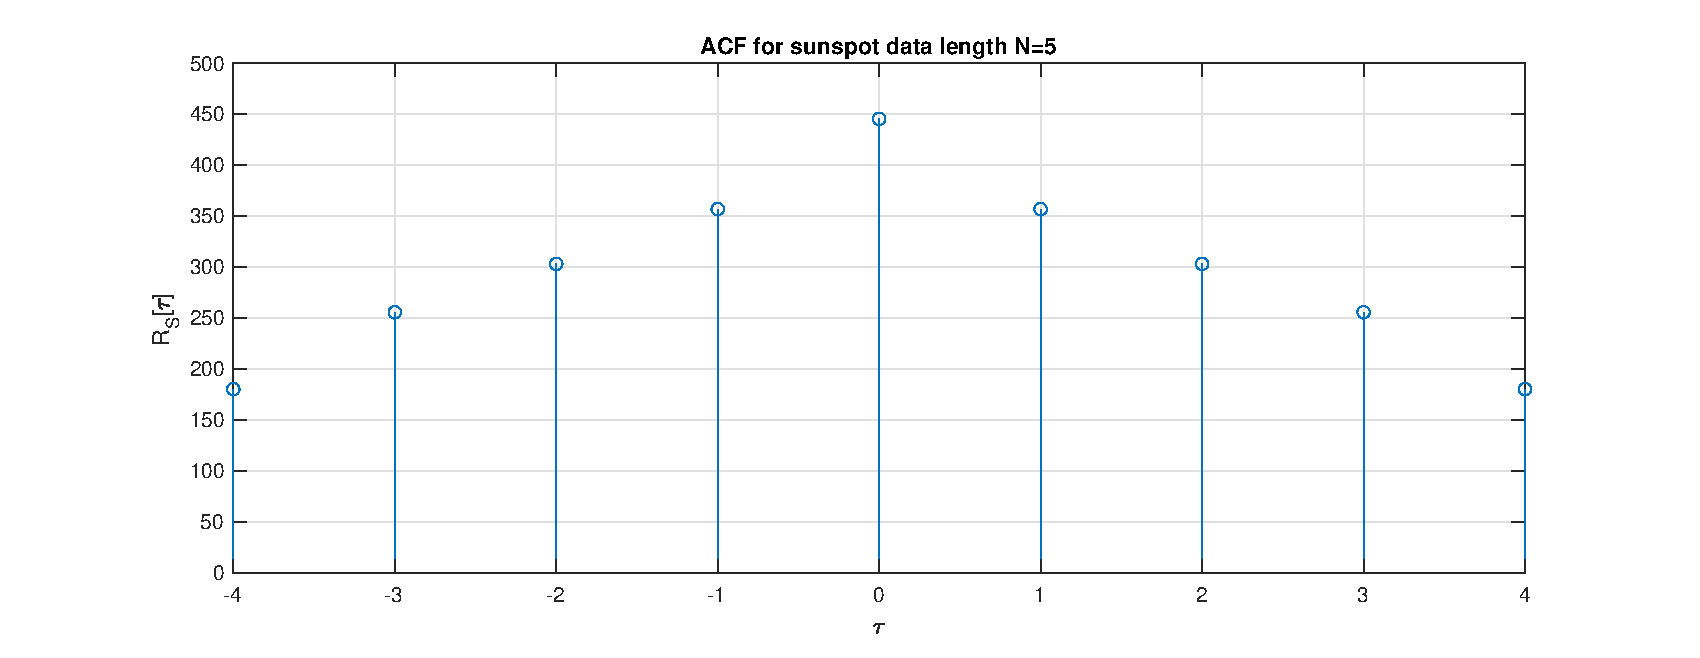
\includegraphics[width=\linewidth]{assignment2figs/acf_sun5.eps}
  \caption{ACF for original data, N = 5.}
  \label{fig:rp1mean}
\end{subfigure}\hfil 
\begin{subfigure}{0.5\textwidth}
  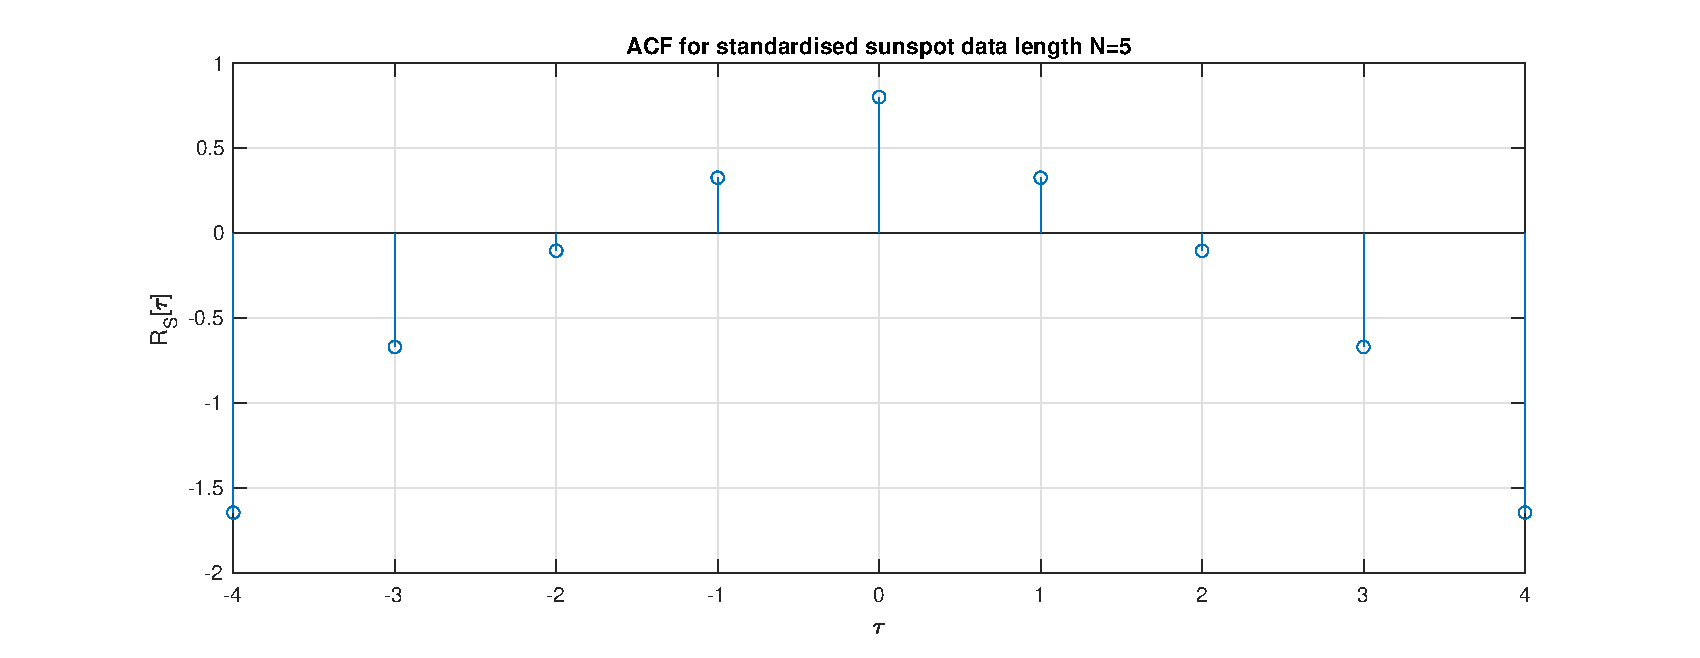
\includegraphics[width=\linewidth]{assignment2figs/acf_sun_norm_5.eps}
  \caption{ACF for standardised data, N = 5.}
  \label{fig:rp1SD}
\end{subfigure}
\medskip
\begin{subfigure}{0.5\textwidth}
  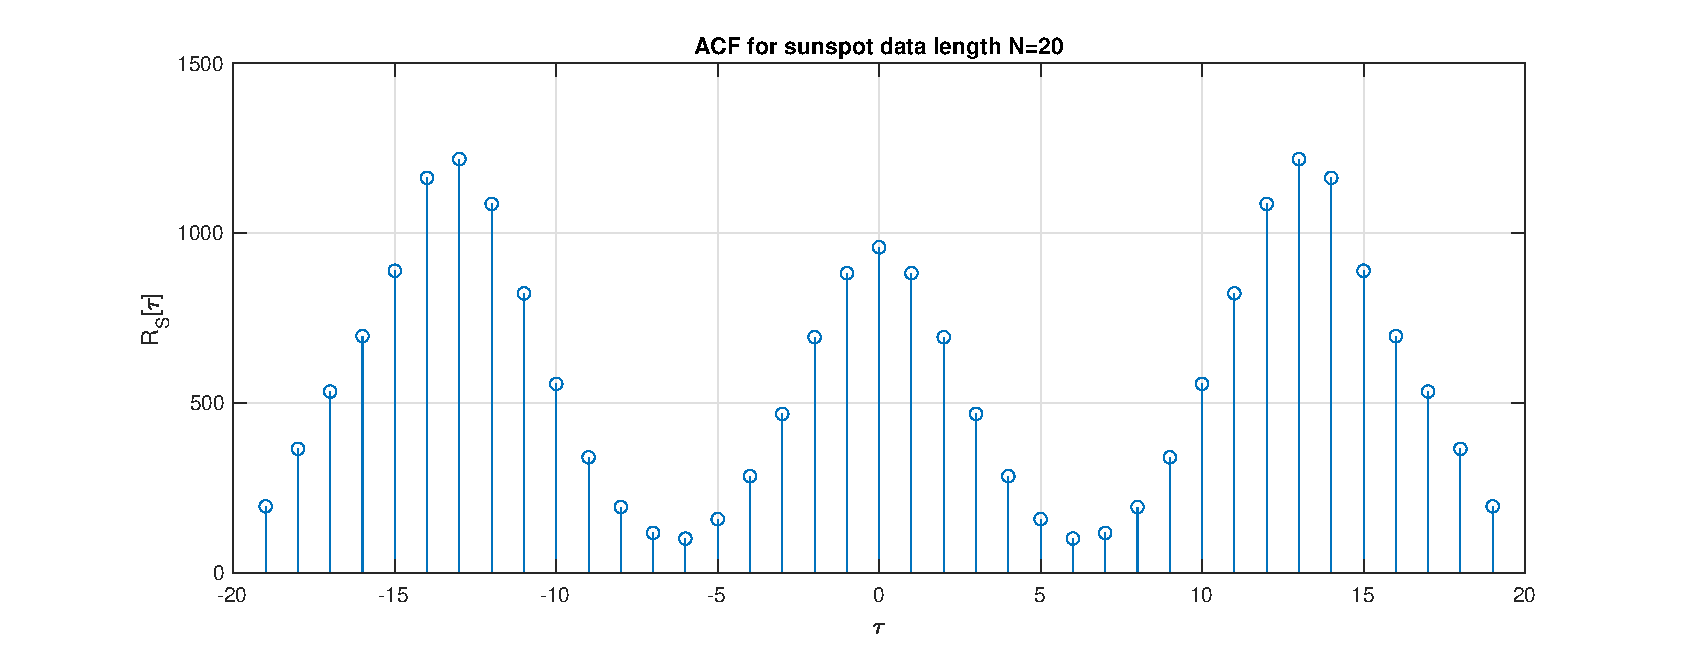
\includegraphics[width=\linewidth]{assignment2figs/acf_sun20.eps}
  \caption{ACF for original data, N = 20.}
  \label{fig:rp2mean}
\end{subfigure}\hfil 
\begin{subfigure}{0.5\textwidth}
  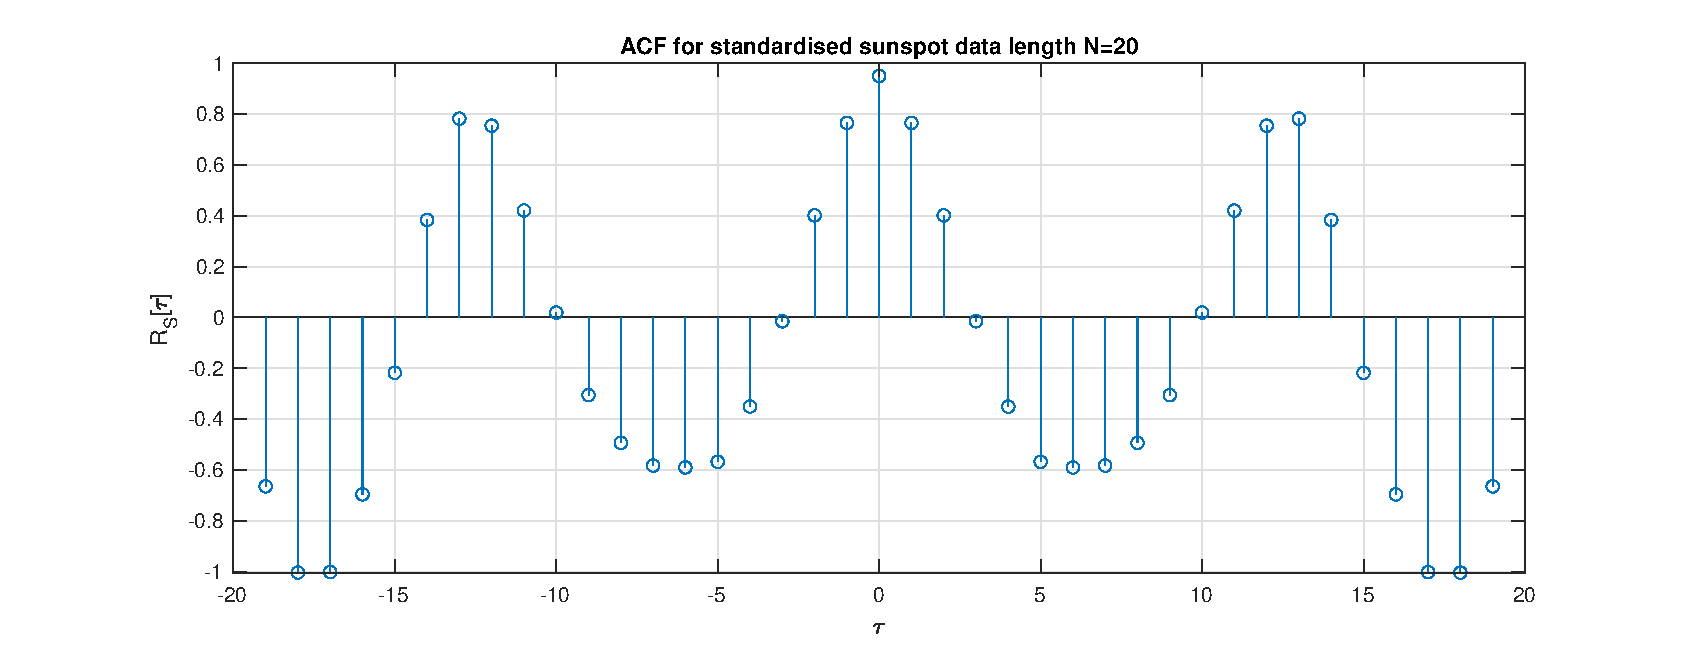
\includegraphics[width=\linewidth]{assignment2figs/acf_sun_norm_20.eps}
  \caption{ACF for standardised data, N = 20.}
  \label{fig:rp2SD}
\end{subfigure}
\medskip
\begin{subfigure}{0.5\textwidth}
  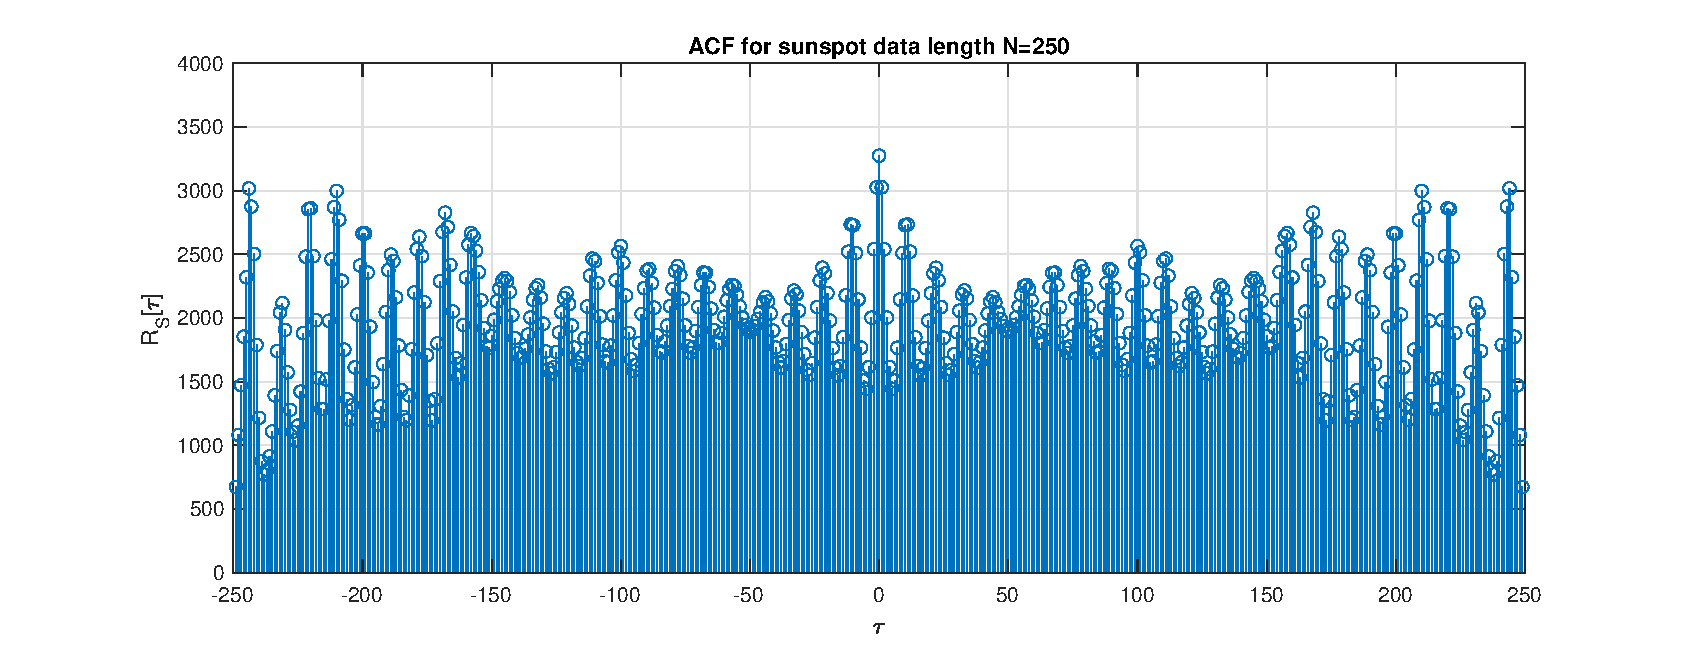
\includegraphics[width=\linewidth]{assignment2figs/acf_sun250.eps}
  \caption{ACF for original data, N = 250.}
  \label{fig:rp3mean}
\end{subfigure}\hfil 
\begin{subfigure}{0.5\textwidth}
  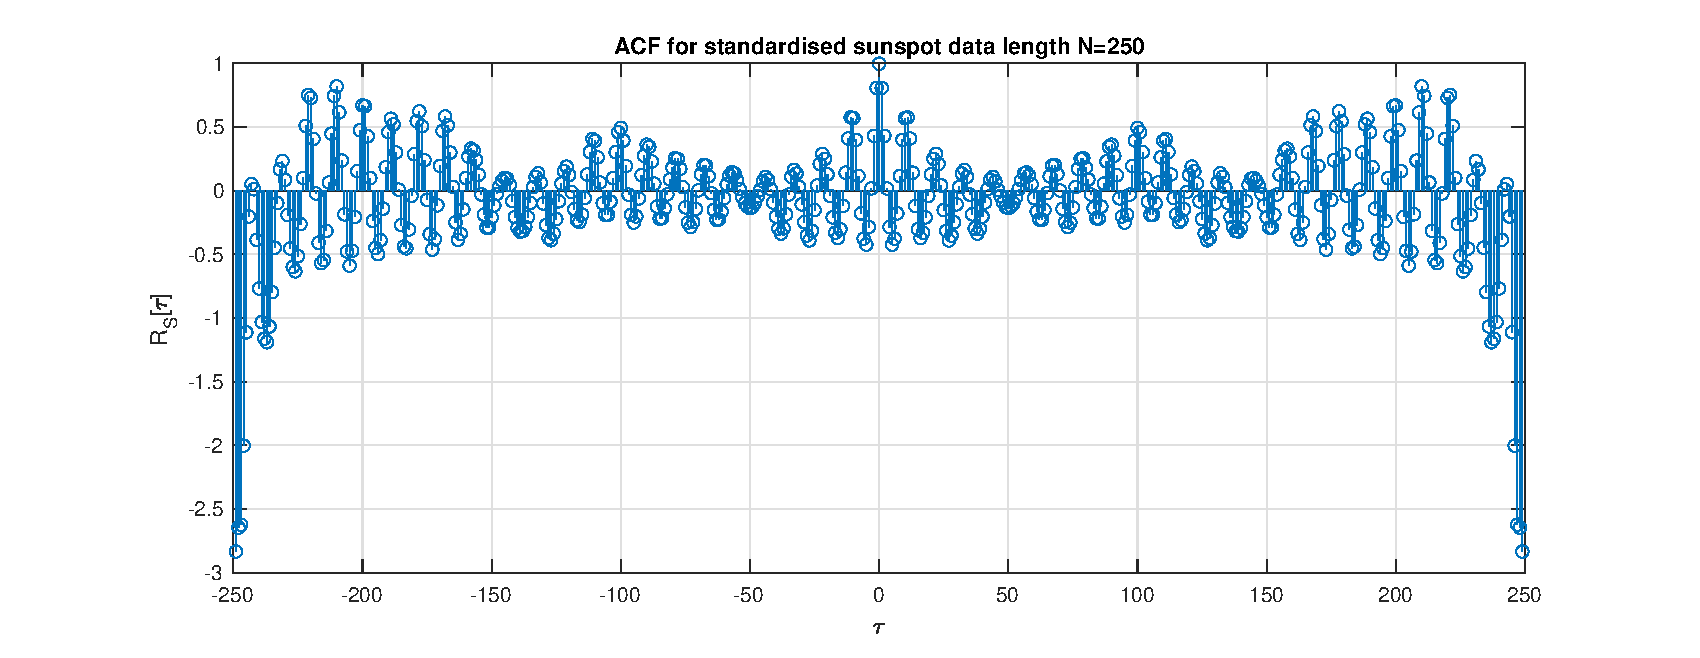
\includegraphics[width=\linewidth]{assignment2figs/acf_sun_norm_250.eps}
  \caption{ACF for standardised data, N = 250.}
  \label{fig:rp3SD}
\end{subfigure}
\caption{ACFs for original and standardised Sunspot data for varying data lengths.}
\label{fig:sun_acfs}
\end{center}
\end{figure}

\noindent
For data length N = 5, the ACF appears to be a triangular function. However, for data length N = 25, the ACF is clearly periodic, with a period of roughly 14 years. For data length N = 250, the ACF still appears to be sinusoidal in nature but is obscured as $|\tau|$ increases. However, within the empirical bound of statistically reliable results $|\tau|<\frac{N}{4}$ identified earlier, the ACF is more clear and appears to be the summation of a sinusoid and a triangular function. There are several irregularities in the ACFs of the original data. Notably, the maximum values are not found at $\tau = 0$. Standardising the data fixes this problem and reveals the self-similarity of the signal more clearly.

\subsubsection{Yule-Walker Equations and PACFs}

Using MATLAB, model coefficients were calculated for a range of model orders using Yule-Walker equations, and are shown in Figure \ref{fig:yulewalker}(a). The PACF of the Sunspot data was also calculated for both the original and standardised values, and is shown in Figure \ref{fig:yulewalker}(b).

\begin{figure}[H]
    \centering
    \subfloat[Yule-Walker model coefficients.]{{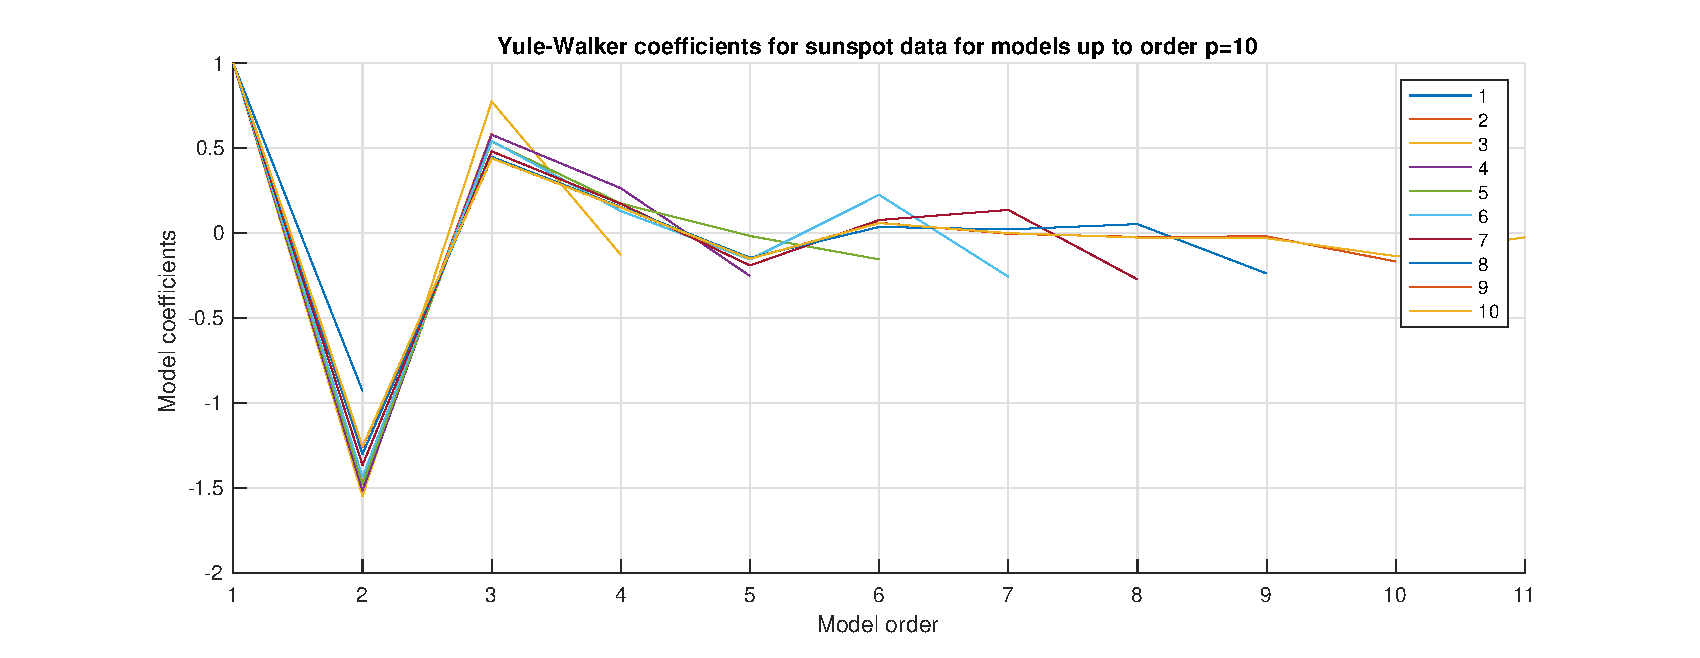
\includegraphics[width=9cm]{assignment2figs/yulewalker.eps}}}
    \subfloat[PACFs for range of model orders]{{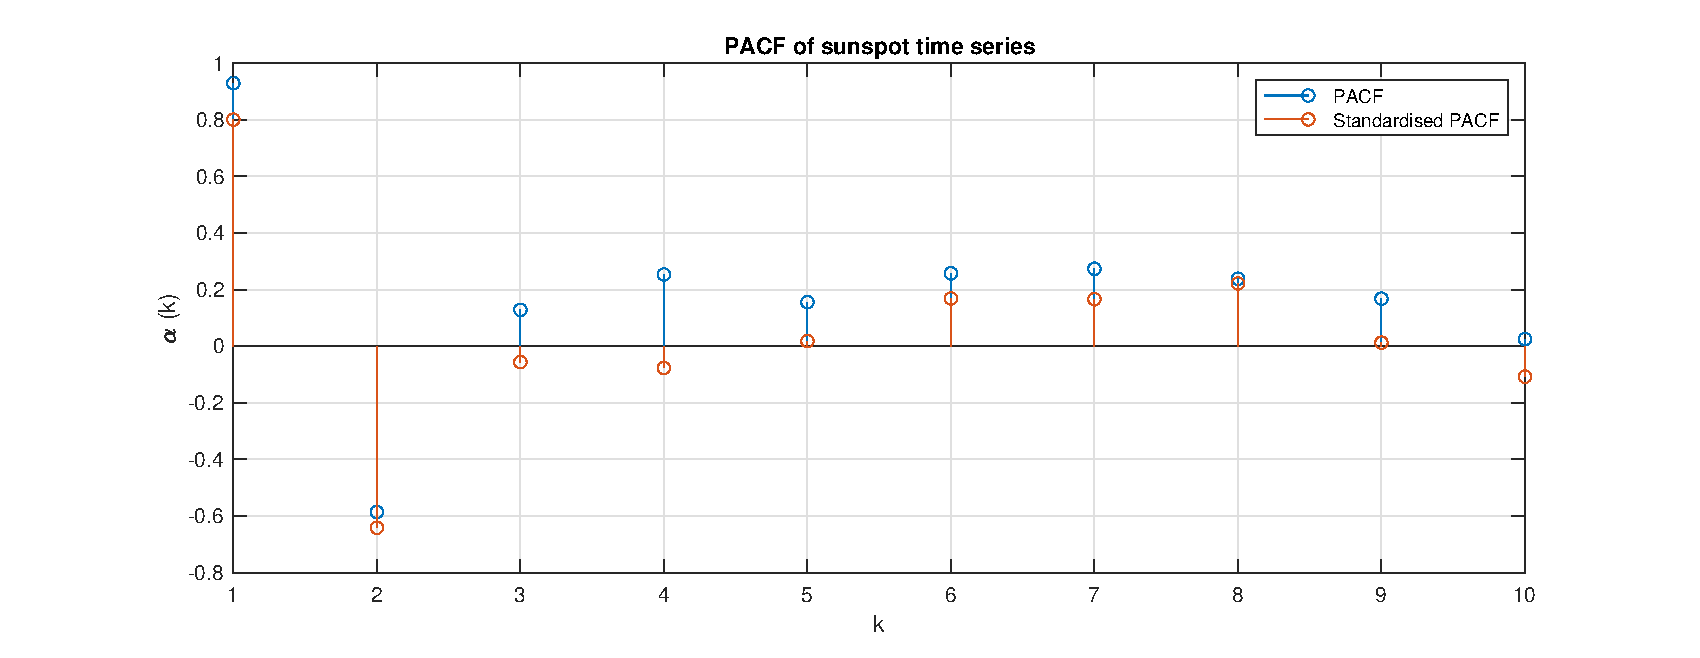
\includegraphics[width=9cm]{assignment2figs/pacfs.eps}}}
    \caption{Statistics for Sunspot data.}
    \label{fig:yulewalker}
\end{figure}

\noindent
Figure \ref{fig:yulewalker}(a) clearly shows that the correct model order is 2, since the coefficients converge to zero for orders above this. Furthermore, the PACF values for orders above 2 are significantly lower, implying that there is little correlation between a given data sample and samples from 3 or more time-steps ago, thus confirming that the correct model order is 2.

\subsubsection{Determining model order}

Minimum description length ($MDL$) and Akaike information criterion ($AIC$) are useful for determining the correct model order when applied to the standardised data. As model order is increased, the loss function decreases but the complexity of the model increases so this does not necessarily imply a better model. $MDL$, $AIC$ and corrected $AIC$ $(AIC_{c})$, defined in Equations \ref{eqn:mdl}-\ref{eqn:aicc} increase in magnitude as order increases, thus their minima can be used to identify the correct model order. 

\begin{equation}
\mathrm{\textit{MDL}} &=\log E_{p}+\frac{p \log N}{N} 
\label{eqn:mdl}
\end{equation}
\begin{equation}
\mathrm{\textit{AIC}} &=\log E_{p}+\frac{2 p}{N}
\label{eqn:aic}
\end{equation}
\begin{equation}
\mathrm{\textit{AIC}_{c}} &=\mathrm{\textit{AIC}}+\frac{2 p(p+1)}{N-p-1}
\label{eqn:aicc}
\end{equation}

\noindent
where $E_{p}$ = loss function, $p$ = number of parameters/ model order and $N$ = number of estimated data points. Plots of these statistics for a range of model orders are displayed in Figure \ref{fig:aic_mdl}.

\begin{figure}[H]
    \centering
    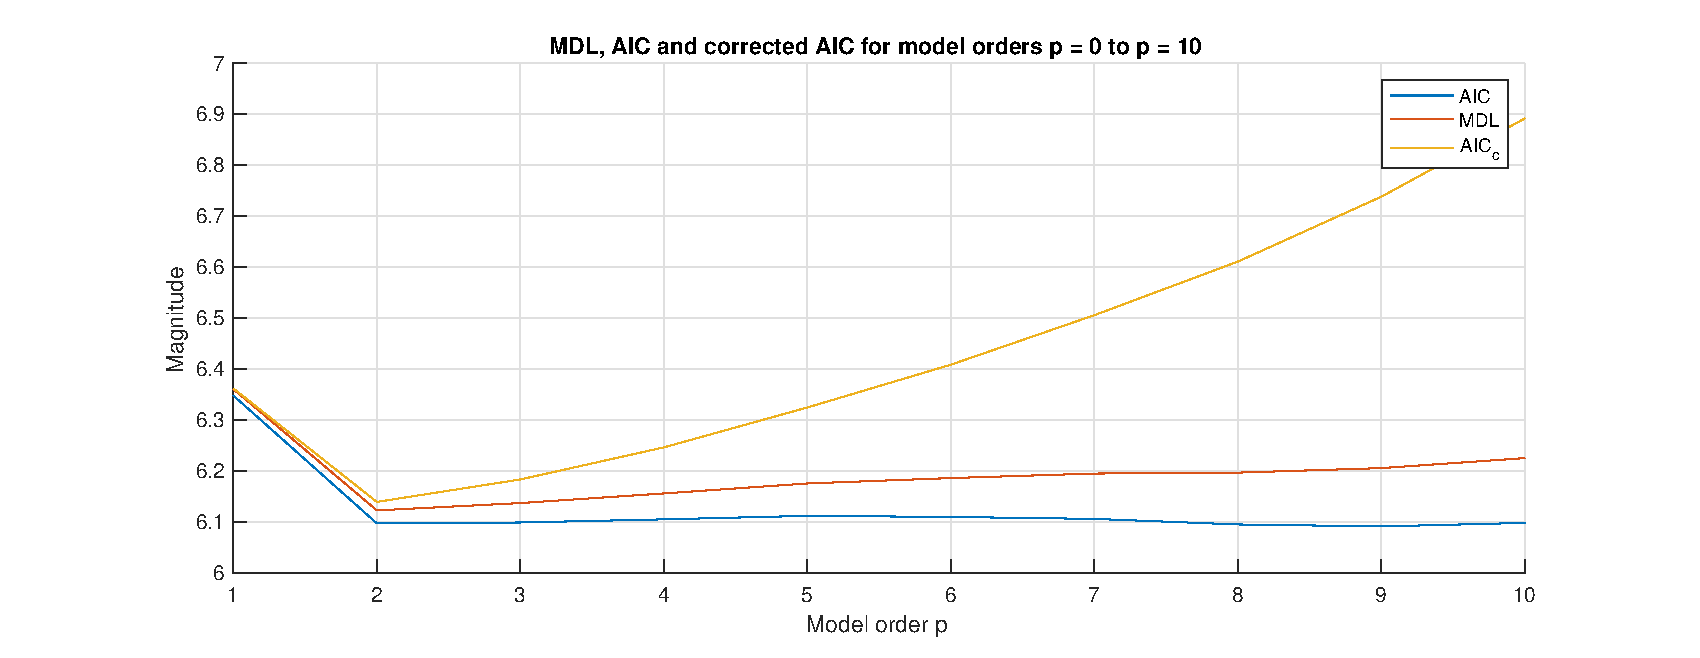
\includegraphics[width=12cm]{assignment2figs/aic_mdl.eps}
    \caption{Statistics for Sunspot time series models.}
    \label{fig:aic_mdl}
\end{figure}

\noindent
The global minima for both $MDL$ and $AIC_{c}$ occurs at p = 2, confirming that the correct model order is 2. Whilst $AIC$ has a local minimum at p = 2, the global minimum is at p = 9. However, this is corrected for by using $AIC_{c}$ so can be ignored. 

\subsubsection{AR Model for Sunspot Time Series}

A comparison was made of AR models for a range of model orders $p$ and prediction horizons $m$. The prediction horizon is defined as the number of time-steps into the future the model is used to predict. Results of this comparison are shown in Figure \ref{fig:sunspotcompound}.

\begin{figure}[H]
    \centering
    \subfloat[][\emph{$p$=1,$m$=1}.]
        {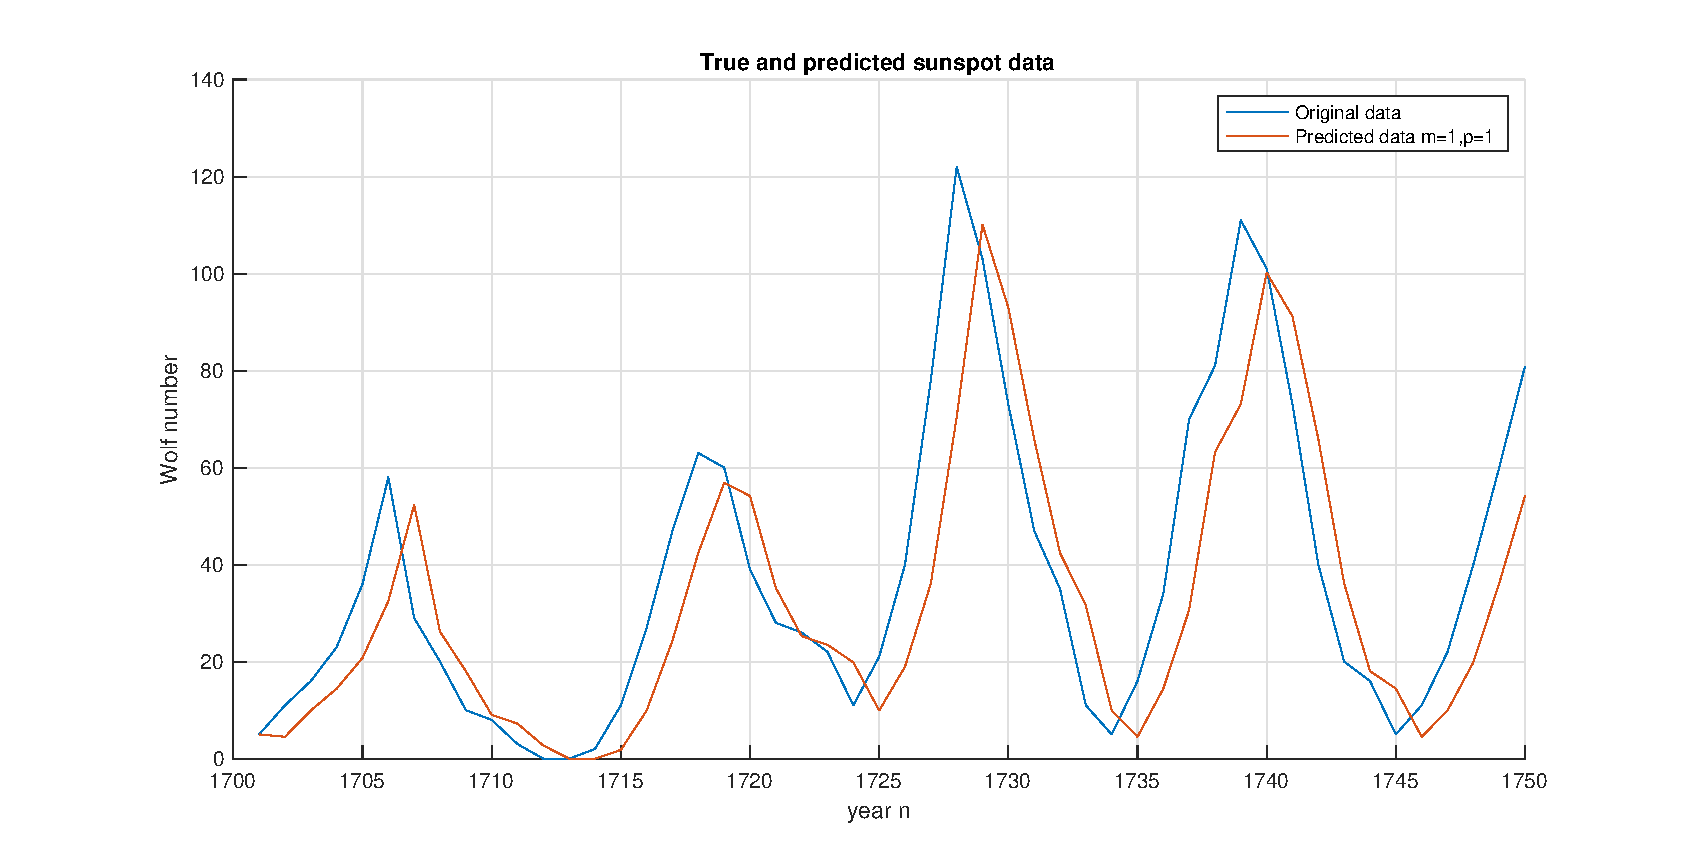
\includegraphics[width=.3\textwidth]{assignment2figs/m1p1.eps}} \quad
    \subfloat[][\emph{$p$=2,$m$=1}.]
        {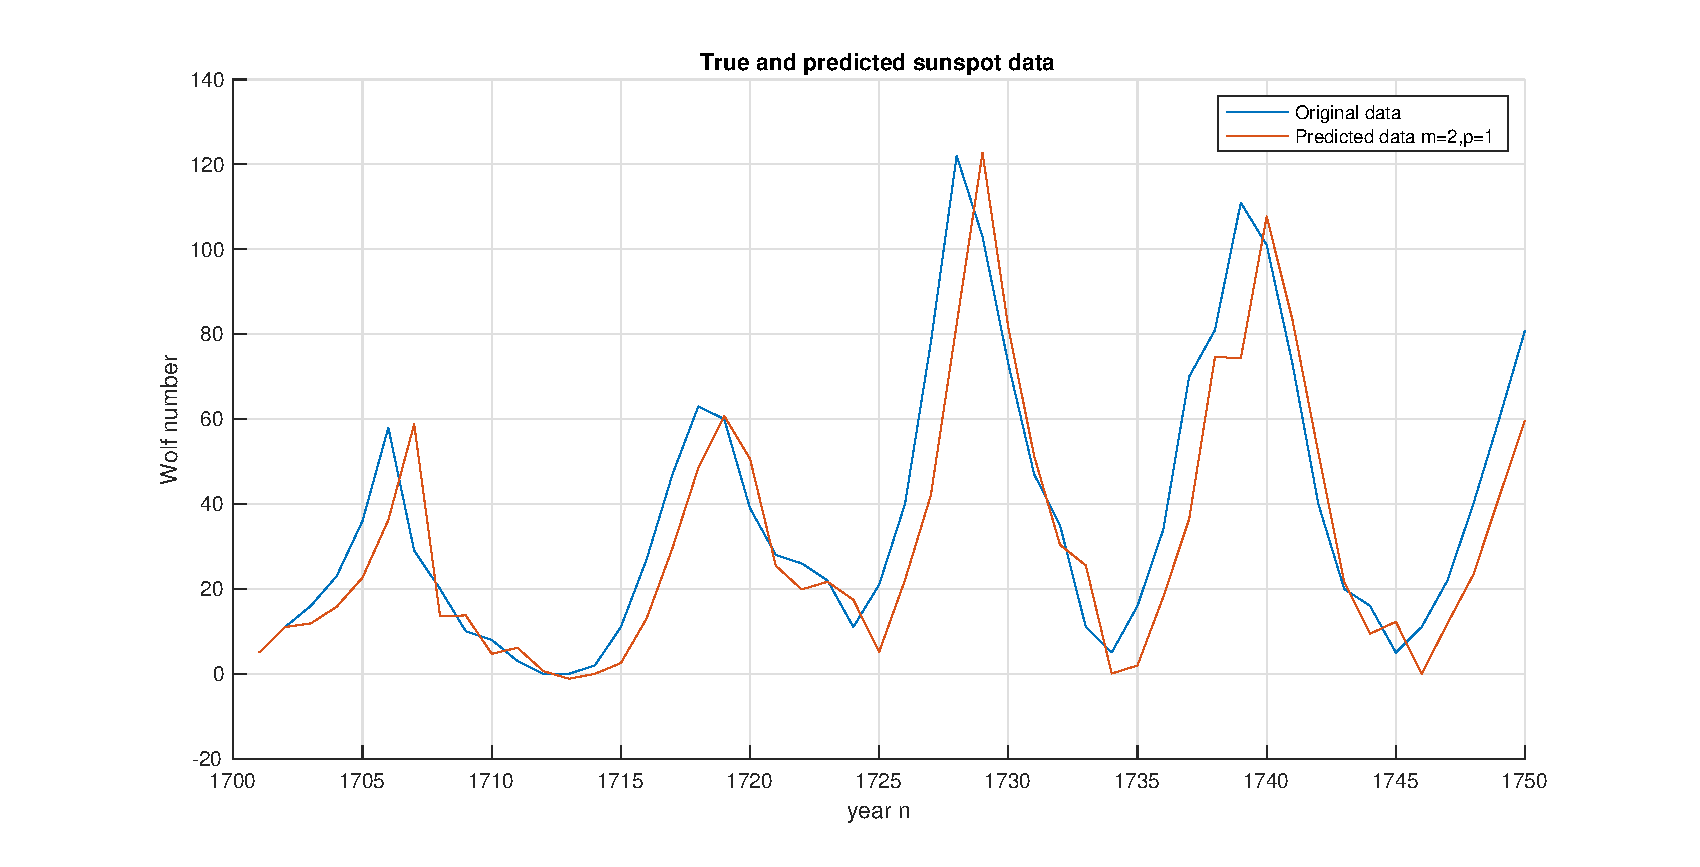
\includegraphics[width=.3\textwidth]{assignment2figs/m2p1.eps}} \quad
    \subfloat[][\emph{$p$=10,$m$=1}.]
        {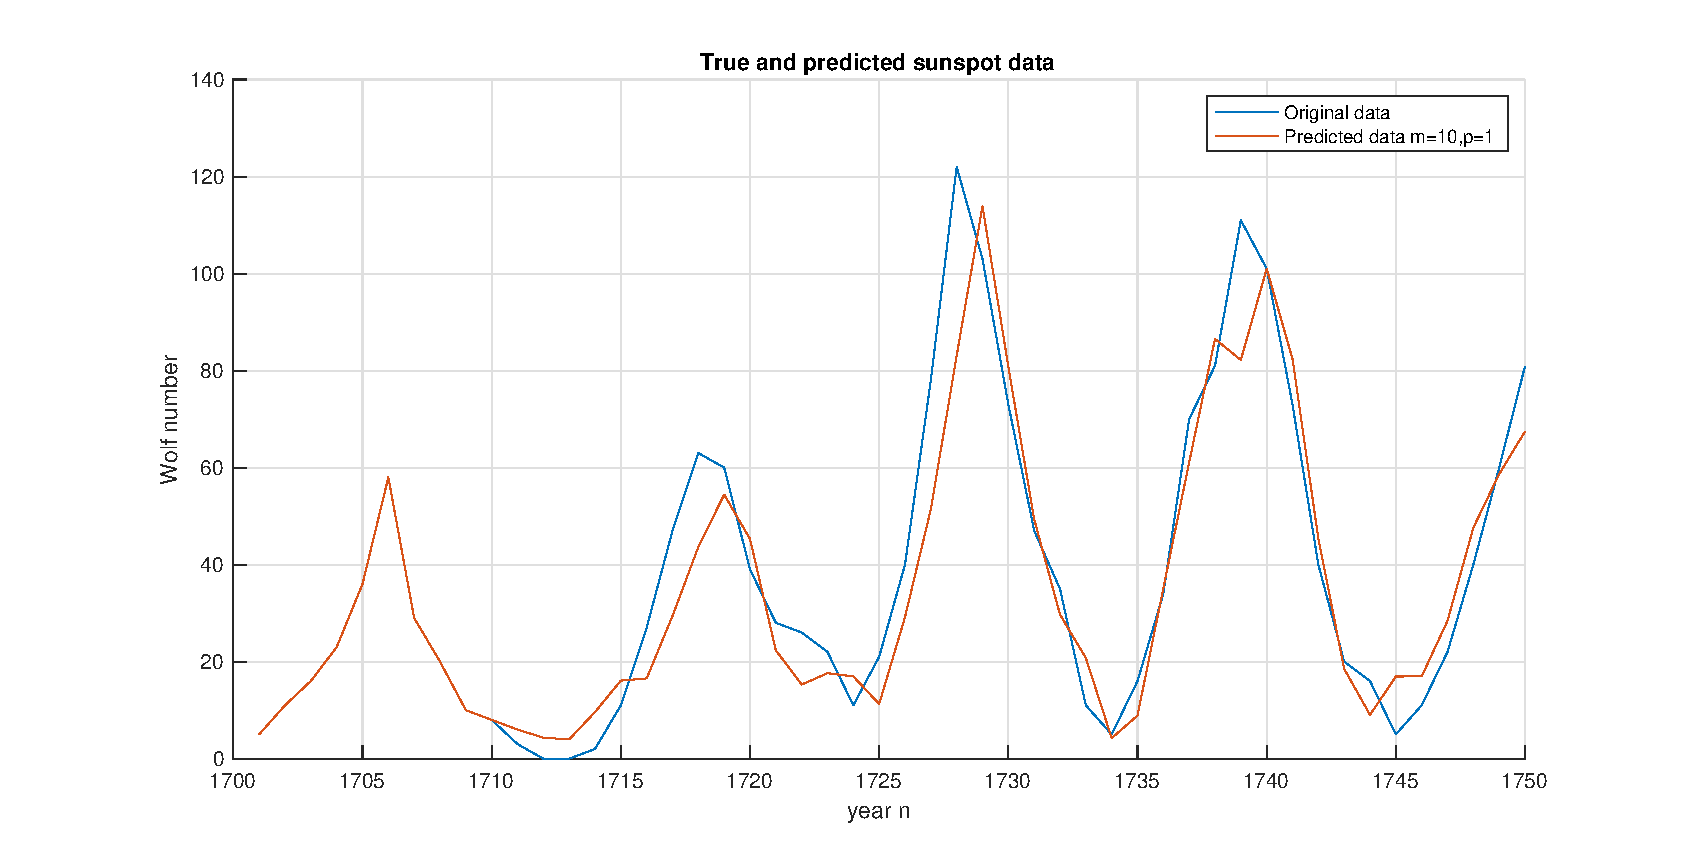
\includegraphics[width=.3\textwidth]{assignment2figs/m10p1.eps}} \\
    \subfloat[][\emph{$p$=1,$m$=2}.]
        {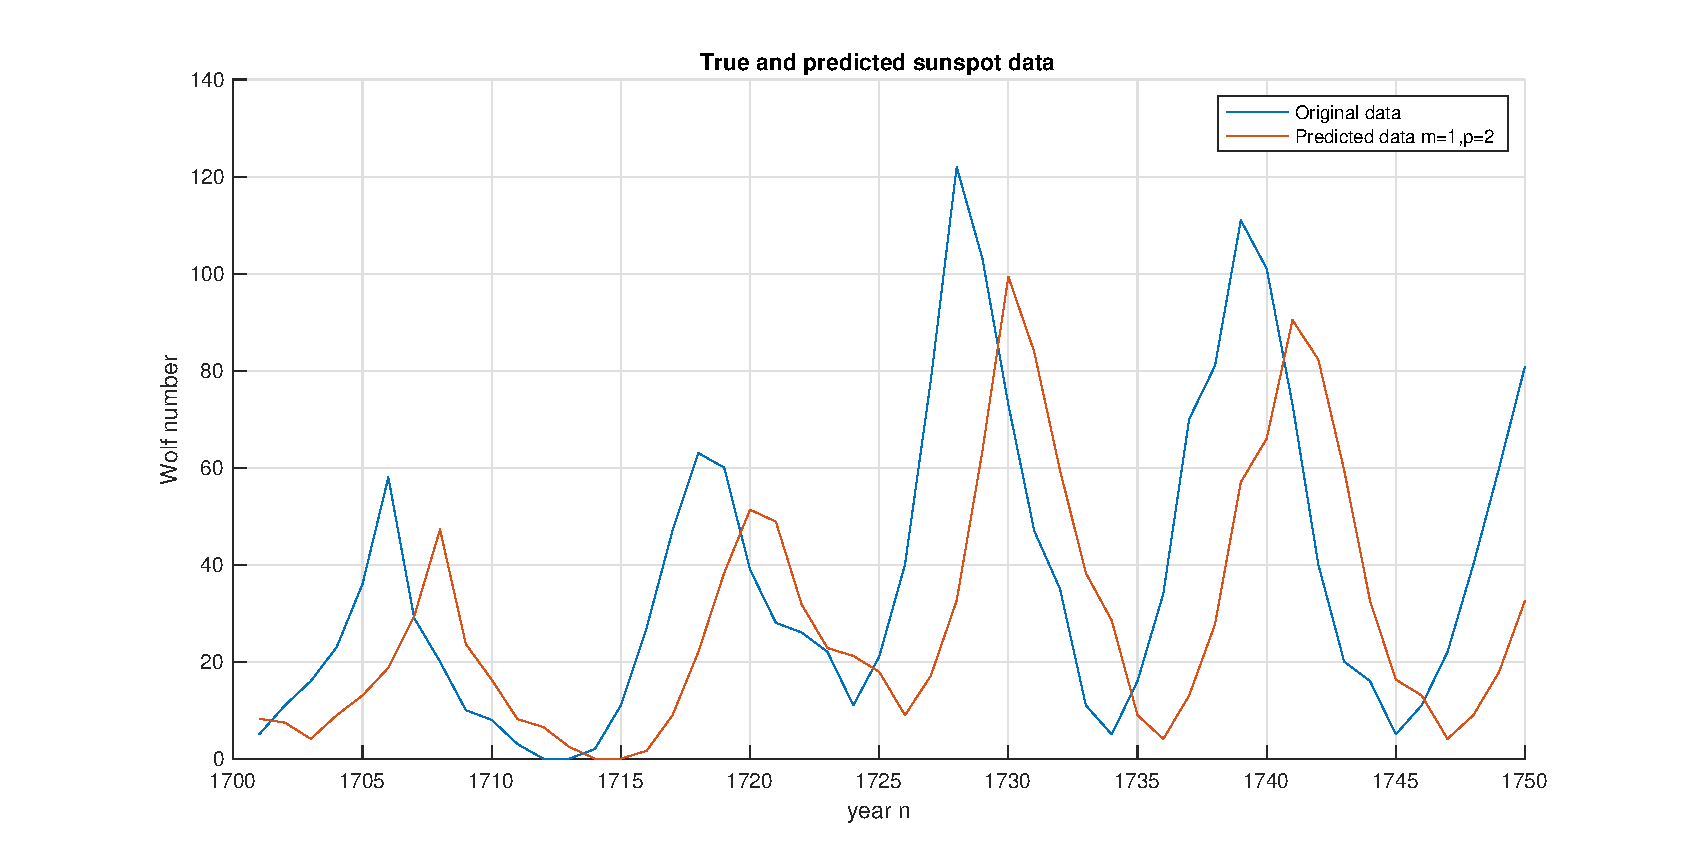
\includegraphics[width=.3\textwidth]{assignment2figs/m1p2.eps}} \quad
    \subfloat[][\emph{$p$=2,$m$=2}.]
        {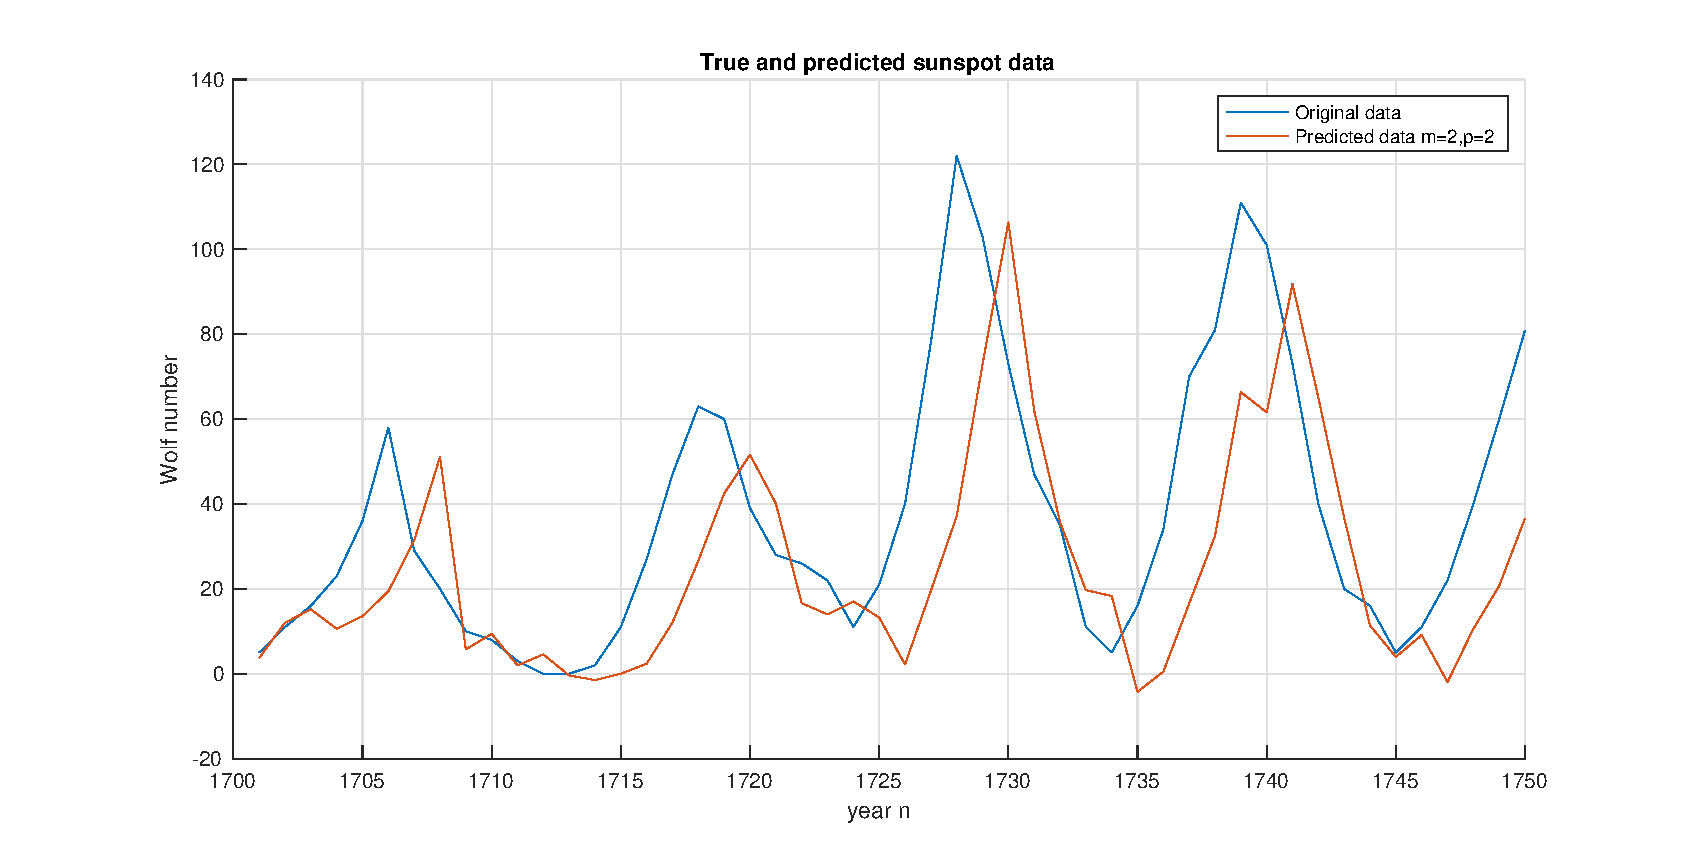
\includegraphics[width=.3\textwidth]{assignment2figs/m2p2.eps}} \quad
    \subfloat[][\emph{$p$=10,$m$=2}.]
        {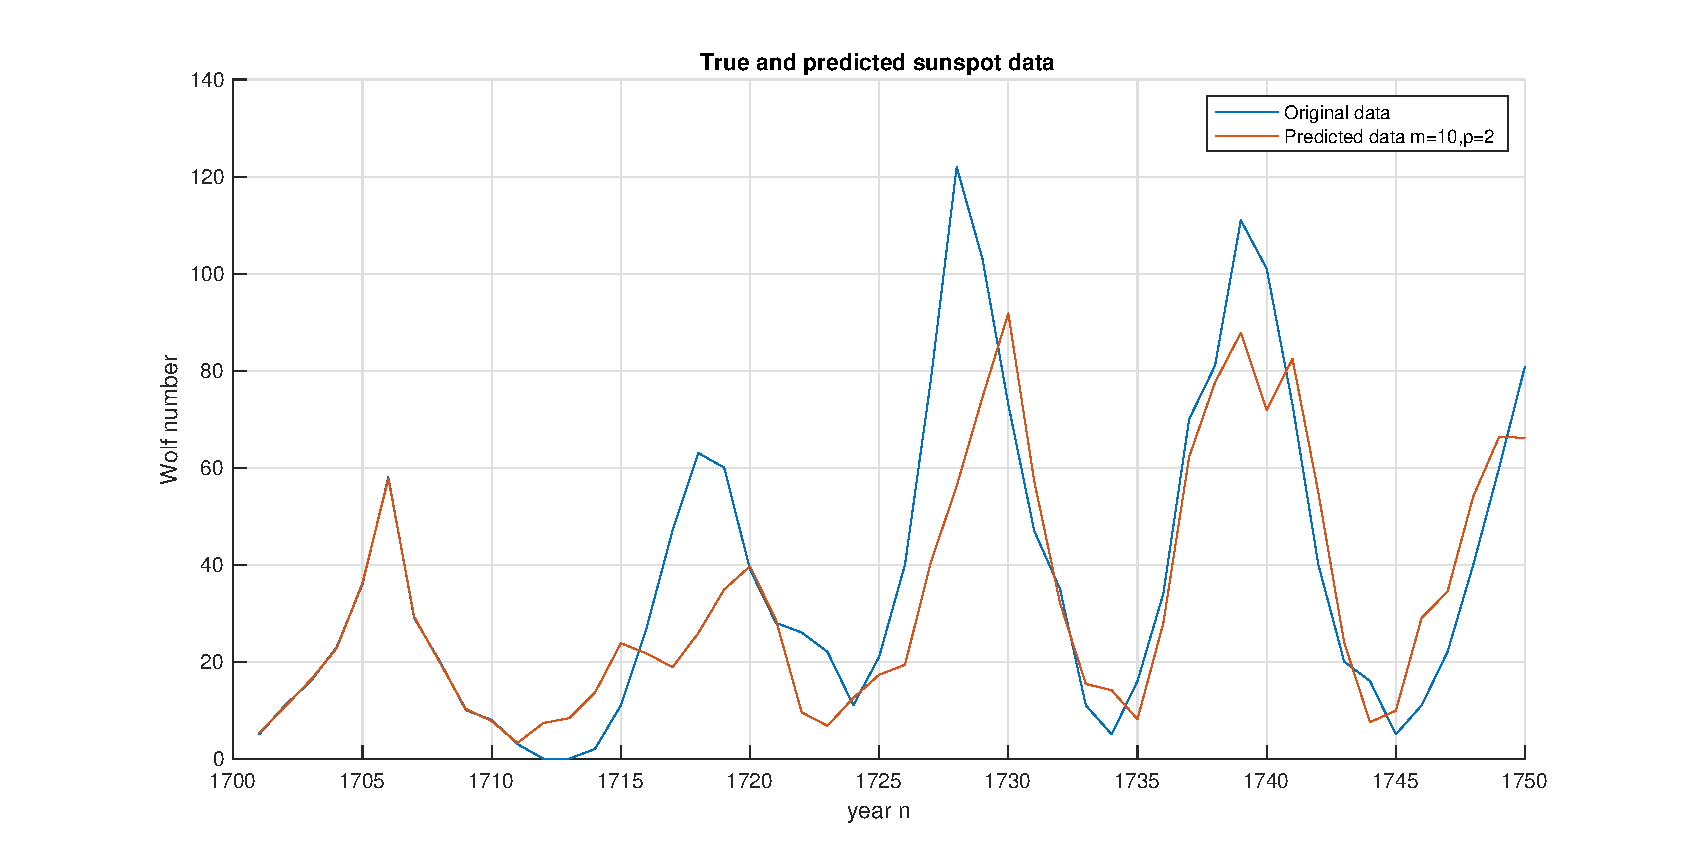
\includegraphics[width=.3\textwidth]{assignment2figs/m10p2.eps}} \\
    \subfloat[][\emph{$p$=1,$m$=5}.]
        {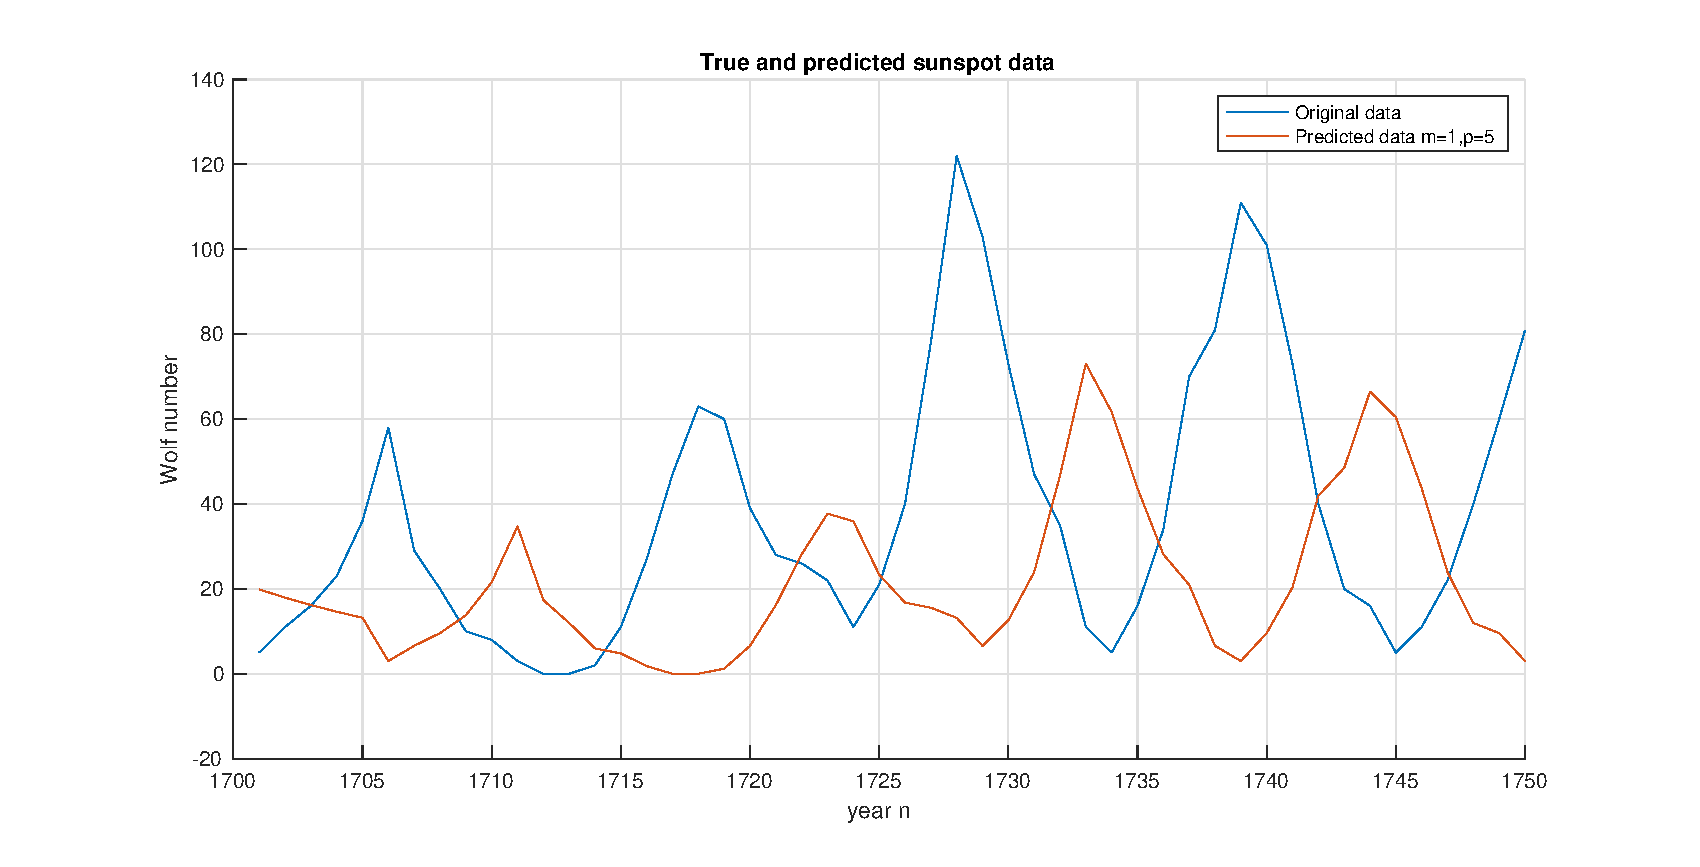
\includegraphics[width=.3\textwidth]{assignment2figs/m1p5.eps}} \quad
    \subfloat[][\emph{$p$=2,$m$=5}.]
        {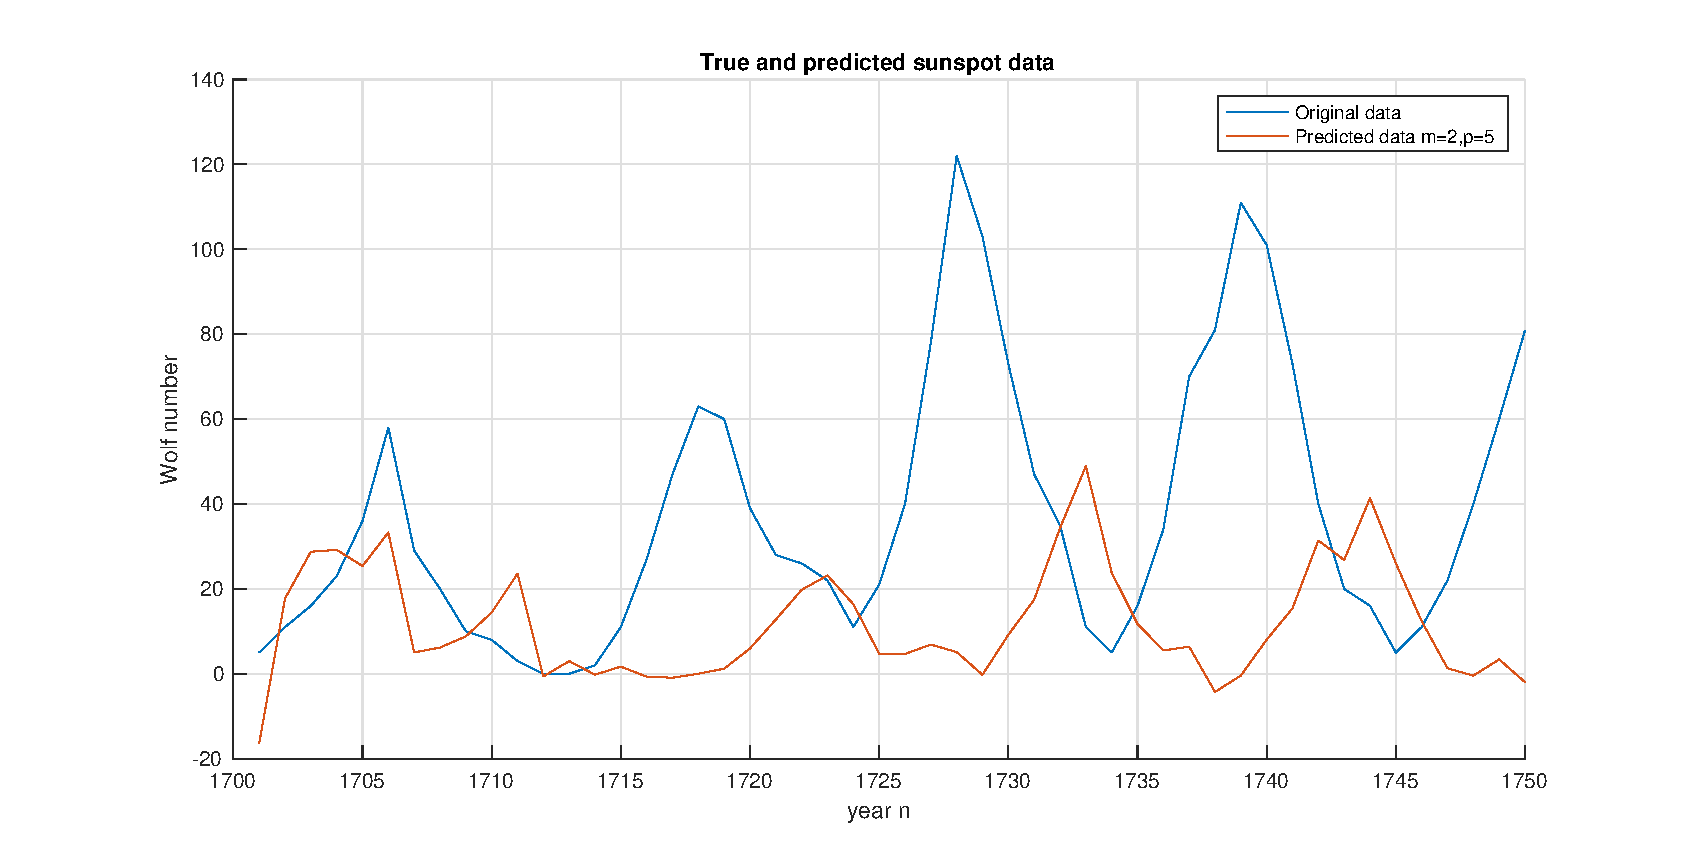
\includegraphics[width=.3\textwidth]{assignment2figs/m2p5.eps}} \quad
    \subfloat[][\emph{$p$=10,$m$=5}.]
        {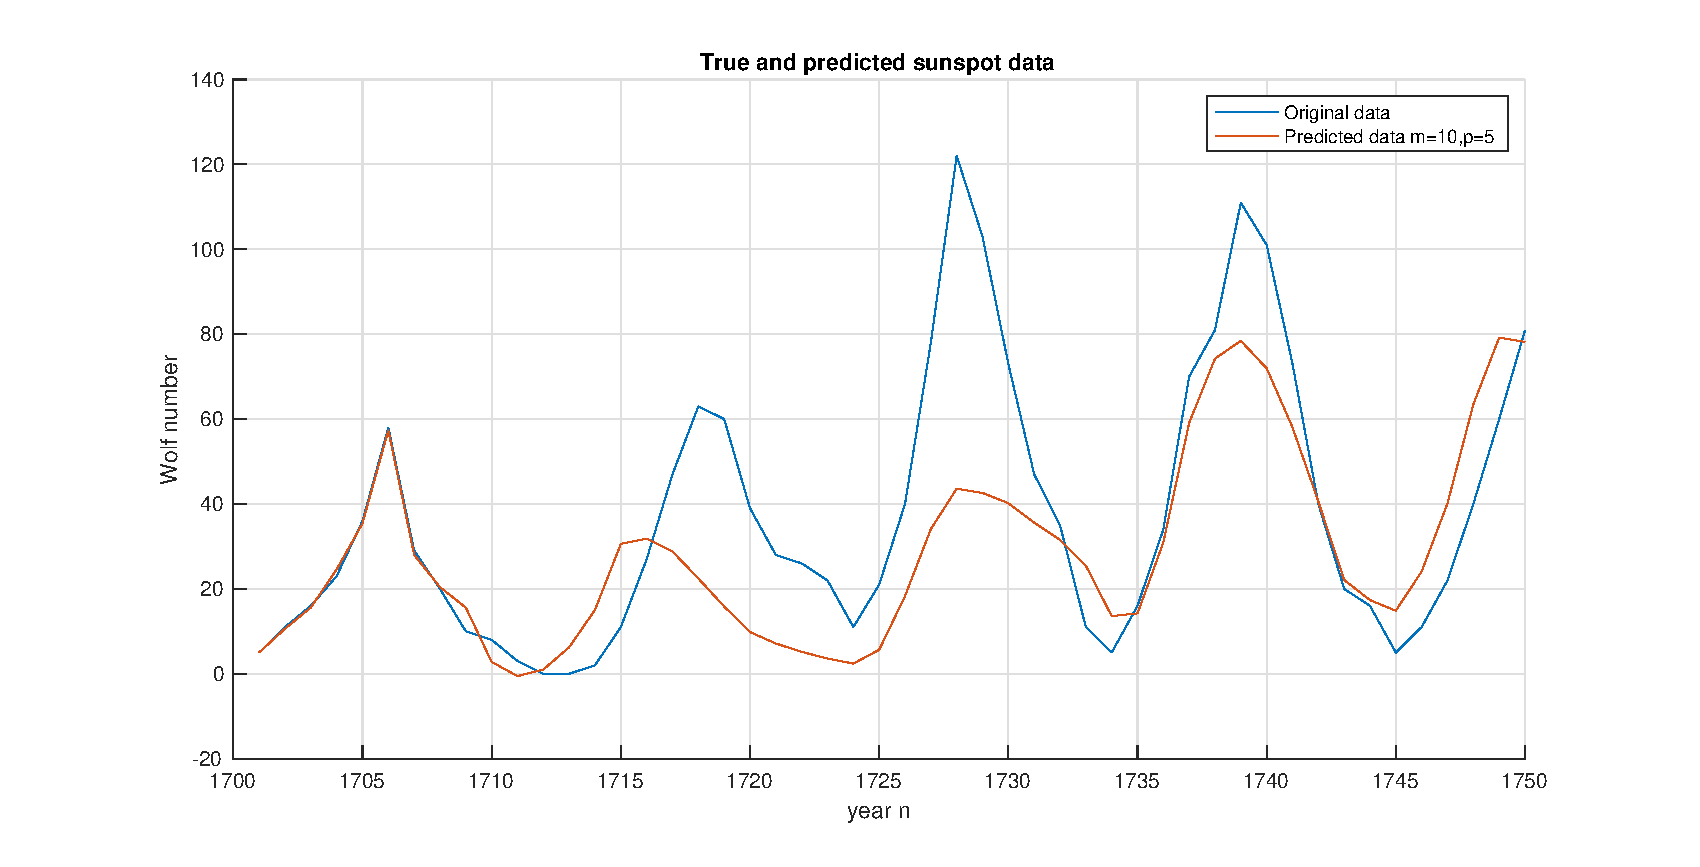
\includegraphics[width=.3\textwidth]{assignment2figs/m10p5.eps}} \\
    \subfloat[][\emph{$p$=1,$m$=10}.]
        {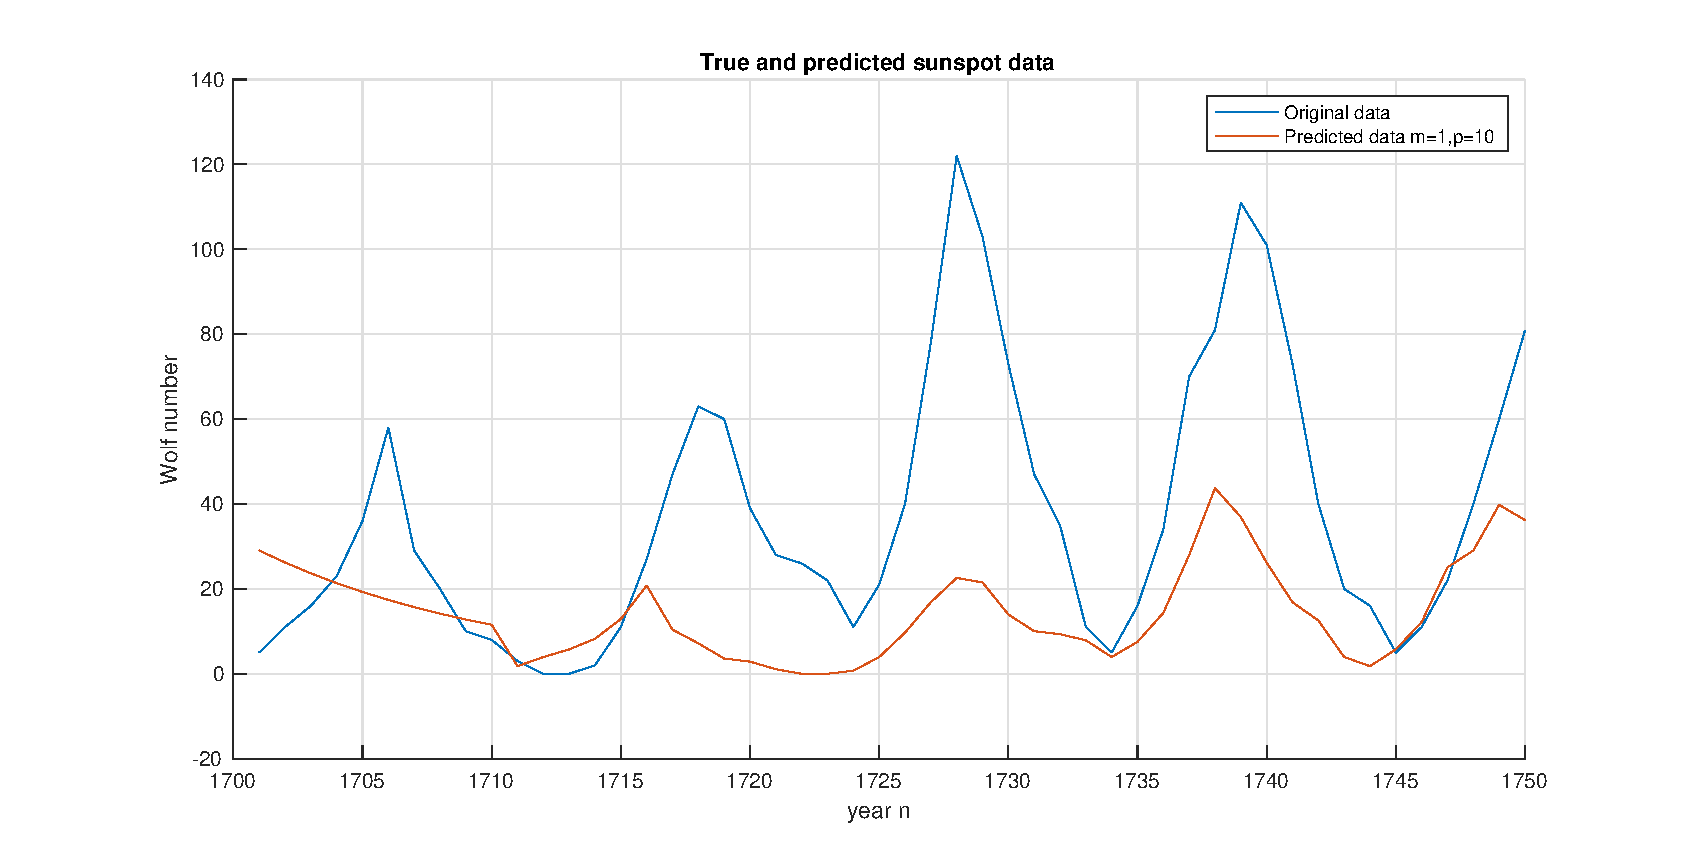
\includegraphics[width=.3\textwidth]{assignment2figs/m1p10.eps}} \quad
    \subfloat[][\emph{$p$=2,$m$=10}.]
        {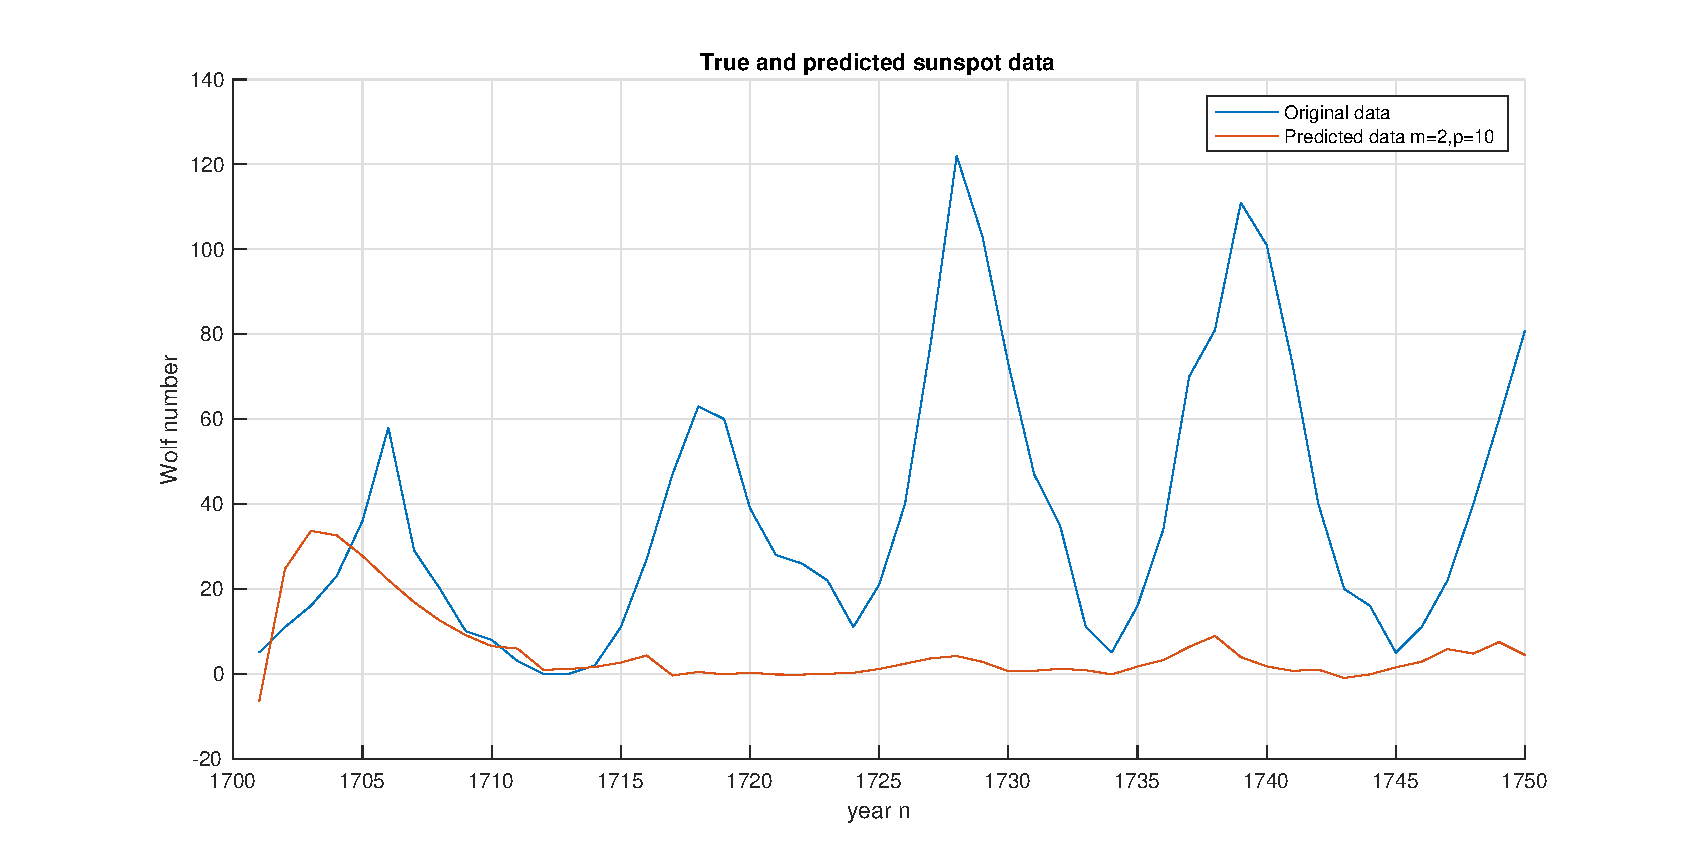
\includegraphics[width=.3\textwidth]{assignment2figs/m2p10.eps}} \quad
    \subfloat[][\emph{$p$=10,$m$=10}.]
        {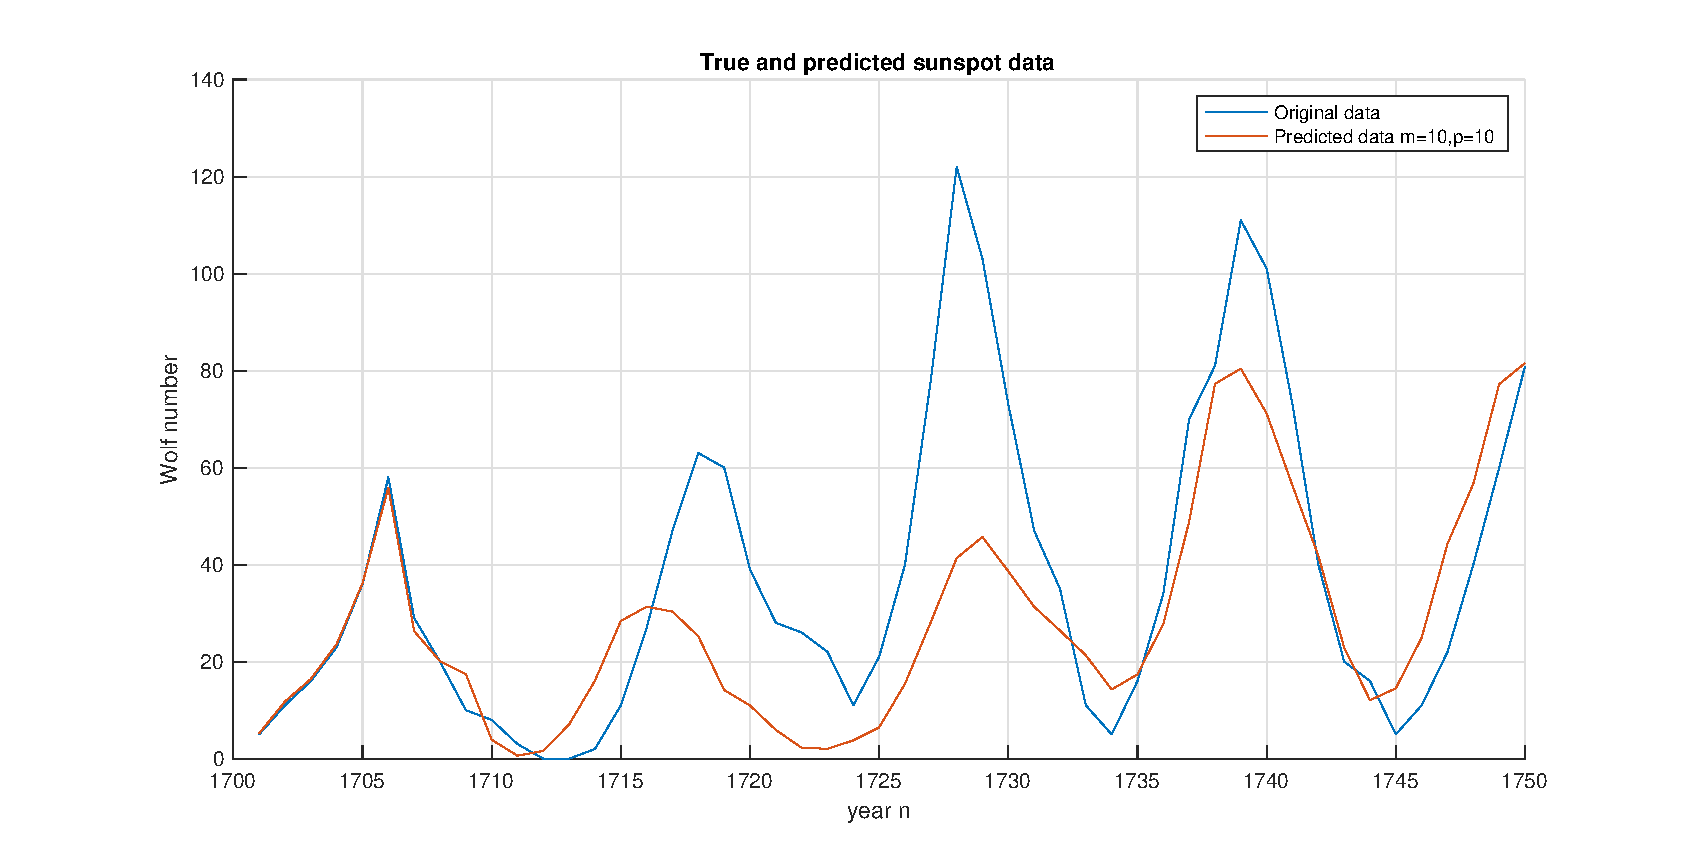
\includegraphics[width=.3\textwidth]{assignment2figs/m10p10.eps}} \\
    \caption{True and predicted data for a range of model orders $p$ and prediction horizons $m$.}
    \label{fig:sunspotcompound}
\end{figure}

\noindent
It is clear from this comparison that increasing the model order increases the temporal precision of the prediction as the time shift between the real and predicted data is significantly less. Increasing the prediction horizon significantly decreases the amplitude of the prediction signal, especially for low order models. This implies that the lower order models AR(1) and AR(2) are not capable of making predictions relatively far in the future (i.e. for a large prediction horizon). This comparison would imply that an AR(10) model is capable of making such predictions accurately, but the computational complexity of the model increases significantly with order and this apparent success in prediction may be an example of model overmodelling. Overmodelling is when more parameters (in this case AR model coefficients) are used for a model than truly describe the process. This results in very low model error, and therefore an apparently accurate model, but will likely result in high prediction error when the model is used for extrapolation. On the contrary, if a model order lower than the true order is chosen, the model will have both high model error and high prediction error, since it cannot make accurate predictions. Minimum prediction error will be found for the true model order, whereas model error will continue to decrease as the model order is increased. This highlights the importance of not using model error as a strict measure of model accuracy, but merely as a rough guide. Testing a model on new data is always necessary in order to build an accurate model, and prediction error should be the primary measure of model accuracy.

% 2.4 Cramer-Rao Lower Bound
\subsection{Cramer-Rao Lower Bound}

Closing prices for the NASDAQ Financial Index from June 2003 to February 2007 were loaded into MATLAB. Analysis was then performed to find the CRLB, a fundamental measure in estimation theory which represents the lower bound oof the variance of unbiased estimators of a deterministic parameter.

\subsubsection{AR(1) model}

Similarly to the Sunspot time series, $MDL$, $AIC$, $AIC_{c}$ and PACF were used to evaluate the sufficiency of AR models of different orders for modelling the NASDAQ time series. The results are displayed in Figure \ref{fig:nasdaq}.

\begin{figure}[H]
    \centering
        \subfloat[$MDL$, $AIC$ and $AIC_{c}$ for NASDAQ data.]{{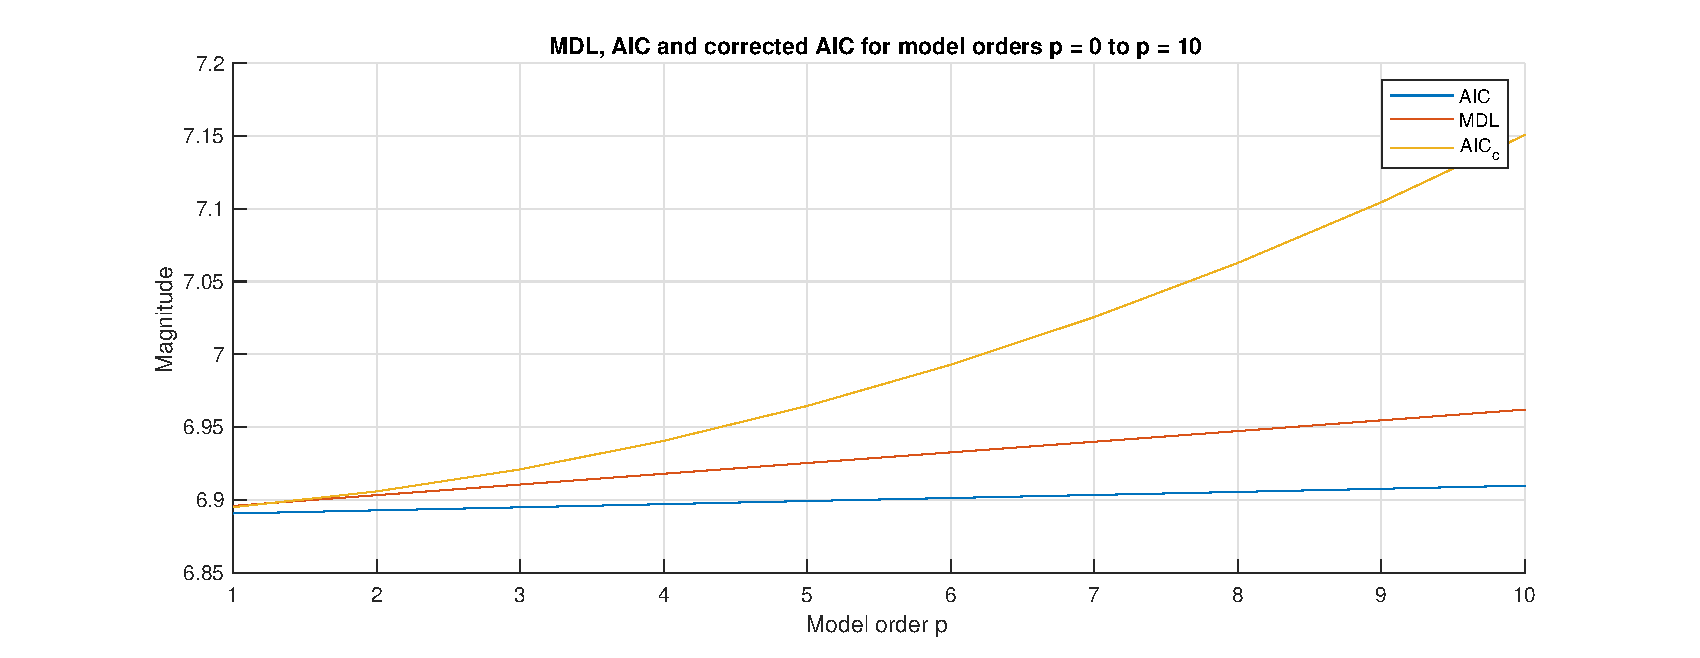
\includegraphics[width=9cm]{assignment2figs/nasdaq_mdl_aic.eps}}}
    \subfloat[PACFs for range of model orders]{{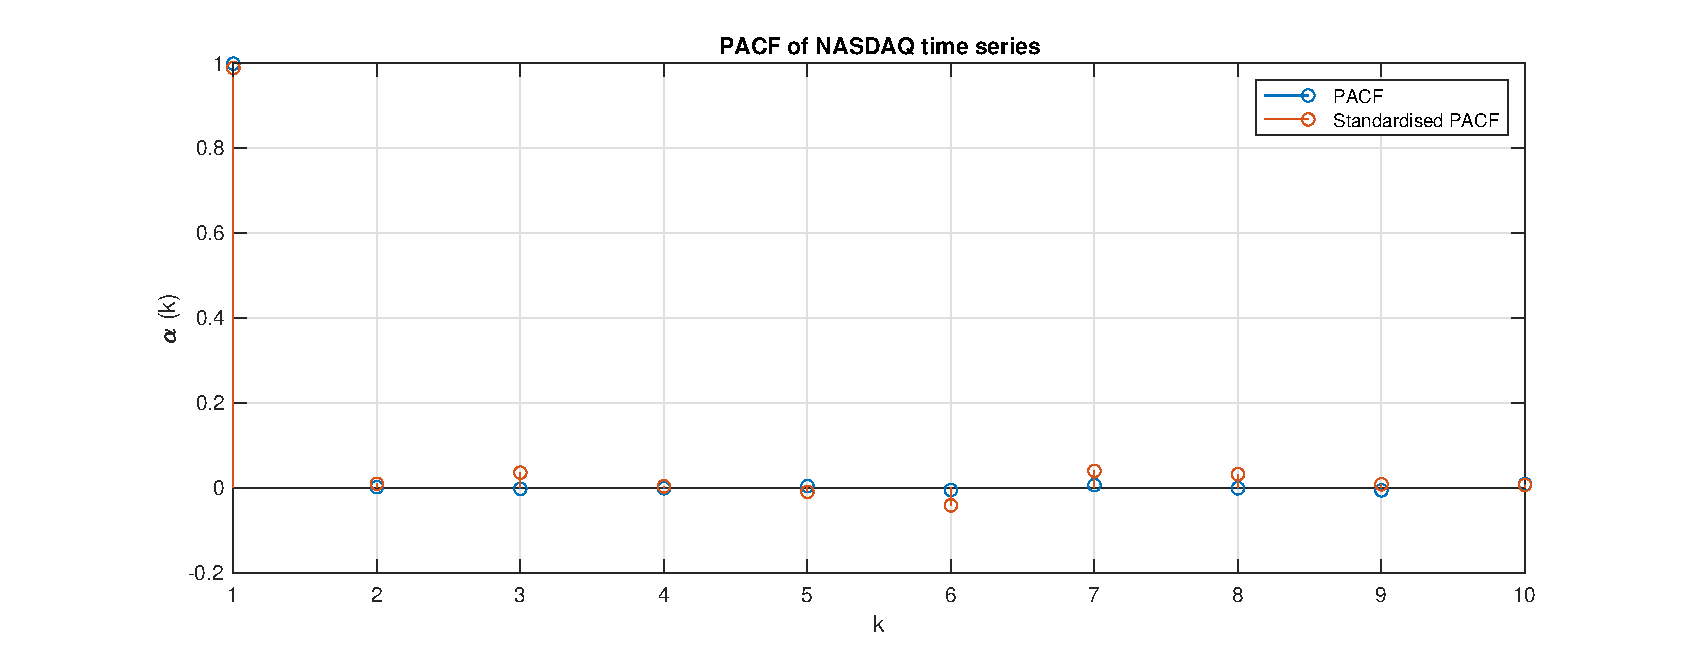
\includegraphics[width=9cm]{assignment2figs/nasdaq_pacf.eps}}}
    \caption{Statistics for NASDAQ data.}
    \label{fig:nasdaq}
\end{figure}

\noindent
It is immediately evident from Figure \ref{fig:nasdaq}(a) that the global minima for all statistics is at p = 1, implying that the correct model order is 1. This is confirmed by the PACF in Figure \ref{fig:nasdaq}(b), which shows by far the highest magnitude for p = 1. This suggests that there is no correlation between samples separated by more than 1 time step, thus an AR(1) model is in fact sufficient to model the NASDAQ time series.

\subsubsection{Fisher Information Matrix}

The asymptotic CRLB of an AR(p) process is given by Equation \ref{eqn:crlb1}.

\begin{equation}
\hat{P}_{X}(f ; \boldsymbol{\theta})=\frac{\hat{\sigma}^{2}}{\left|1-\sum_{m=1}^{p} \hat{a}_{m} e^{-\jmath 2 \pi f m}\right|^{2}}
\label{eqn:crlb1}
\end{equation}

\noindent
where $\hat{\sigma}^{2}$ is the estimated value of the driving noise variance and $p$ is the order. The elements of the Fisher Information Matrix, $\boldsymbol{I}(\boldsymbol{\theta})$ are given by Equation \ref{eqn:fim} where $\boldsymbol{\theta}=\left[a_{1}, \sigma^{2}\right]$, whilst $\ln \left[\hat{P}_{X}(f ; \boldsymbol{\theta})\right]$ is given by Equation \ref{eqn:ln}.

\begin{equation}
[\mathbf{I}(\boldsymbol{\theta})]_{i j}=\frac{N}{2} \int_{-\frac{1}{2}}^{\frac{1}{2}} \frac{\partial \ln \left[\hat{P}_{X}(f ; \boldsymbol{\theta})\right]}{\partial \theta_{i}} \frac{\partial \ln \left[\hat{P}_{X}(f ; \boldsymbol{\theta})\right]}{\partial \theta_{j}} d f
\label{eqn:fim}
\end{equation}

\begin{equation}
\ln \left[\hat{P}_{X}(f ; \boldsymbol{\theta})\right]=\ln \left[\hat{\sigma}^{2}\right]-\ln \left[1-\sum_{m=1}^{p} \hat{a}_{m} e^{-\jmath 2 \pi f m}\right]-\ln \left[1-\sum_{m=1}^{p} \hat{a}_{m} e^{\jmath 2 \pi f m}\right]
\label{eqn:ln}
\end{equation}

\noindent
In order to find $[\mathbf{I}(\boldsymbol{\theta})]_{2 2}$, p=1 is assumed and Equation \ref{eqn:ln} is substituted into Equation \ref{eqn:fim}, along with \boldsymbol{\theta} as below.

\begin{equation}
[\boldsymbol{I}(\boldsymbol{\theta})]_{22}=\frac{N}{2} \int_{-\frac{1}{2}}^{\frac{1}{2}} \frac{\partial \ln \left[\hat{P}_{X}(f ; \boldsymbol{\theta})\right]}{\partial \sigma^{2}} \frac{\partial \ln \left[\hat{P}_{X}(f ; \boldsymbol{\theta})\right]}{\partial \sigma^{2}} d f
\end{equation}

\begin{equation}
\frac{N}{2} \int_{-\frac{1}{2}}^{\frac{1}{2}} \frac{1}{\sigma^{4}} d f
\end{equation}
\begin{equation}
\frac{N}{2}\left[\frac{1}{\sigma^{4}}\right]_{-\frac{1}{2}}^{\frac{1}{2}}
\end{equation}
\begin{equation}
\frac{N}{2}\left[\frac{1}{2 \sigma^{4}}-\left(-\frac{1}{2 \sigma^{4}}\right)\right]
\end{equation}
\begin{equation}
[\boldsymbol{I}(\boldsymbol{\theta})]_{22}=\frac{N}{2 \sigma^{4}}
\end{equation}

\noindent
Since $[\boldsymbol{I}(\boldsymbol{\theta})]_{11}, [\boldsymbol{I}(\boldsymbol{\theta})]_{12}$ and $[\boldsymbol{I}(\boldsymbol{\theta})]_{21}$ were given, we can conclude that the Fisher Information Matrix is given by Equation
\ref{eqn:fisher}.

\begin{equation}
[\boldsymbol{I}(\boldsymbol{\theta})]=\left(\begin{array}{cc}
\frac{N r_{x x}(0)}{\sigma^{2}} & 0 \\
0 & \frac{N}{2 \sigma^{4}}
\end{array}\right)
\label{eqn:fisher}
\end{equation}

\subsubsection{CRLB of variance}

The CRLB is given by Equation \ref{eqn:crlb2}.

\begin{equation}
\textit{var}\left(\hat{\theta}_{i}\right) \geq\left[I^{-1}(\theta)\right]_{i i}
\label{eqn:crlb2}  
\end{equation}

\noindent
Therefore, the CRLB for the given matrix is calculated as below. 
\begin{equation}
\textit{var}\left(\hat{\sigma}^{2}\right)=\textit{var}\left(\hat{\theta}_{2}\right) \geq\left[I^{-1}(\theta)\right]_{22}
\end{equation}
\begin{equation}
\textit{var}\left(\hat{\sigma}^{2}\right) \geq\left(\frac{N}{2 \sigma^{4}}\right)^{-1} 
\end{equation}
\begin{equation}
\textit{var}\left(\hat{\sigma}^{2}\right) \geq \frac{2 \sigma^{4}}{N}
\end{equation}

\noindent
The other bound to be proved is given by \ref{eqn:bound2}.

\begin{equation}
\textit{var}\left(\hat{a}_{1}\right)=\textit{var}\left(\hat{\theta}_{1}\right) \geq\left[\boldsymbol{I}^{-1}(\boldsymbol{\theta})\right]_{11}
\label{eqn:bound2}
\end{equation}

\noindent
Using the Fisher Information Matrix, this can be rewritten as Equation \ref{eqn:rewrite}.

\begin{equation}
\textit{var}\left(\hat{a}_{1}\right) \geq \frac{\sigma^{2}}{N r_{x x}[0]}
\label{eqn:rewrite}
\end{equation}

\noindent
$r_{x x}[0] = \frac{\sigma_{w}^{2}}{1-a_{1}^{2}}$, therefore Equation \ref{eqn:rewrite} can be rewritten to obtain the desired result below.

\begin{equation}
\textit{var}\left(\hat{a}_{1}\right) & \geq \frac{\sigma^{2}}{N} \frac{1-a_{1}^{2}}{\sigma^{2}}
\end{equation}
\begin{equation}
\textit{var}\left(\hat{a}_{1}\right) & \geq \frac{1}{N}\left(1-a_{1}^{2}\right)
\label{eqn:finalres}
\end{equation}

\noindent
Letting N = number of data points and $\sigma^{2}$ = driving noise variance, heatmaps were plotted ranging between 1 and 1001 in increments of 50, and are shown in Figure \ref{fig:heatmaps}.

\begin{figure}[H]
    \centering
        \subfloat[Heatmap for $\hat{a_{1}}$.]{{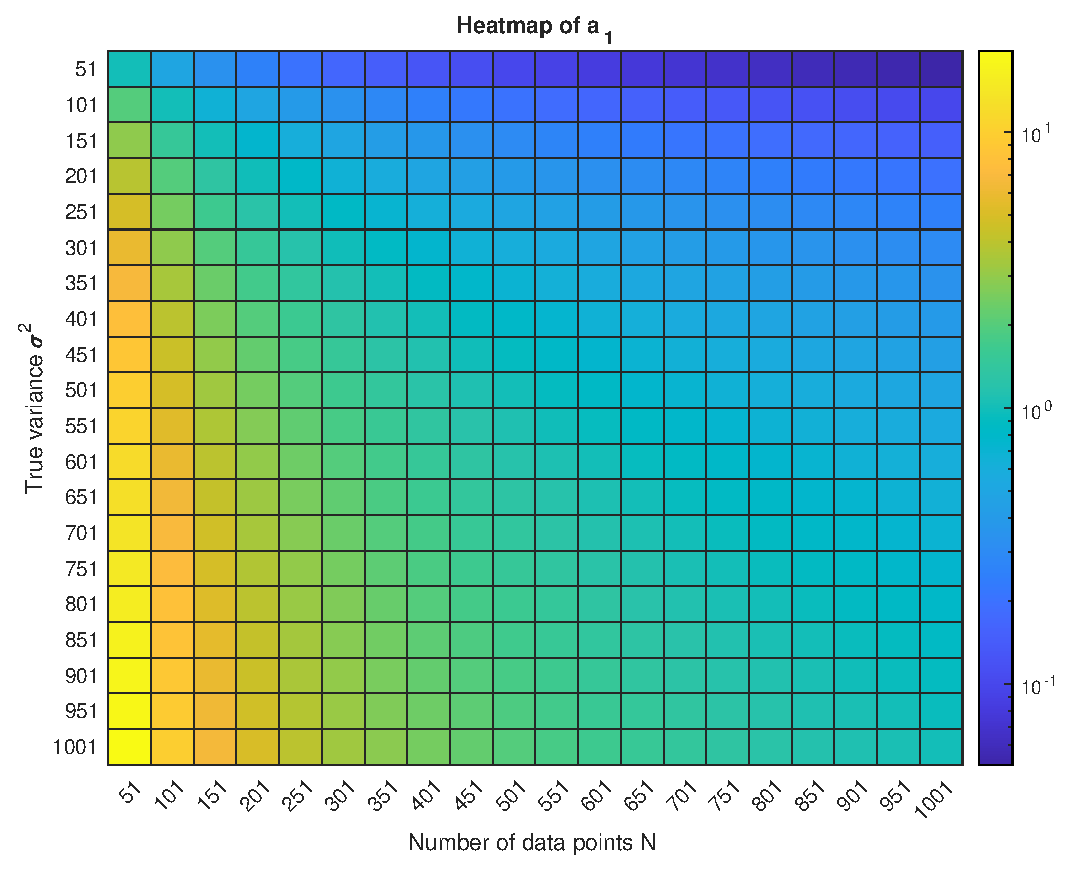
\includegraphics[width=7cm]{assignment2figs/heatmap_a.eps}}}
    \subfloat[Heatmap for noise variance $\hat{\sigma^{2}}$.]{{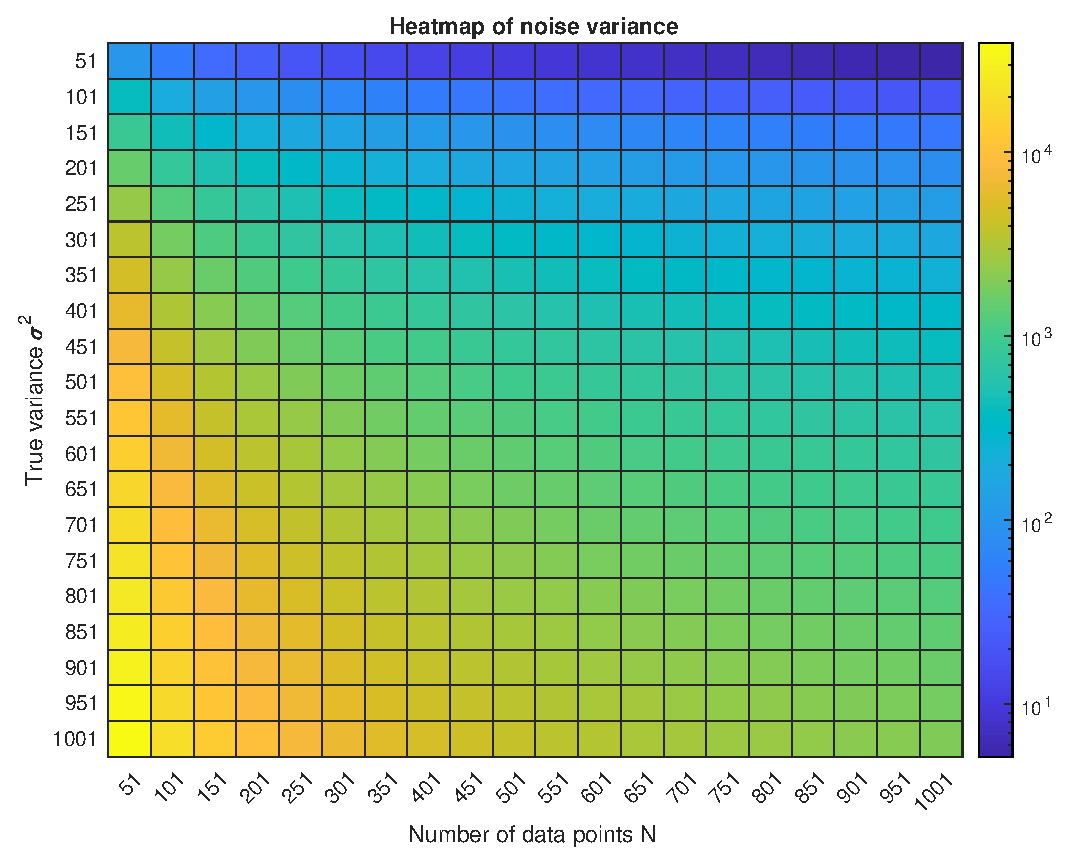
\includegraphics[width=7cm]{assignment2figs/heatmap_var.eps}}}
    \caption{Heatmaps illustrating variation in CRLB.}
    \label{fig:heatmaps}
\end{figure}

\noindent
The largest CRLB for both $\hat{a_{1}}$ and $\hat{\sigma^{2}}$ is found where the noise variance is highest and the number of data points used for calculation is lowest. This can be explained by the fact that $
\textit{var}\left(\hat{\sigma}^{2}\right) \propto \sigma^{4} \text {,  } \textit{var}\left(\hat{\sigma}^{2}\right) \propto \frac{1}{N} \text { and } \textit{var}\left(\hat{a_{1}}\right) \propto \frac{1}{N}
$. Using the result derived above, $var(\hat{a_{1}})$ can be calculated. From the NASDAQ data, the coefficient $a_{1}$ of the AR(1) model is -0.999. Substituting this into Equation \ref{eqn:finalres}, the result is obtained $var(\hat{a_{1}}) = 2.16 \times 10^{−6}$.

\subsubsection{Bound in terms of A(f)}

From the CRLB, it can be shown that 

\begin{equation}
\textit{var}\left(\hat{P}_{X}(f ; \boldsymbol{\theta})\right) \geq \frac{\partial \hat{P}_{X}(f ; \boldsymbol{\theta})^{T}}{\partial \boldsymbol{\theta}} \boldsymbol{I}^{-1}(\theta) \frac{\partial \hat{P}_{X}(f ; \boldsymbol{\theta})}{\partial \boldsymbol{\theta}}
\label{eqn:crlb9}
\end{equation}

\noindent
Letting $A(f)=1-a_{1} e^{-j 2 \pi f}$ and defining $\frac{\partial P_{X}(f ; \theta)}{\partial \theta}$ as in Equation \ref{eqn:flo}.

\begin{equation}
\frac{\partial \hat{P}_{X}(f ; \boldsymbol{\theta})}{\partial \boldsymbol{\theta}}=\left(\frac{2 e^{-j 2 * t_{f}} \sigma^{2}}{|A(f)|^{3}} \frac{1}{\left|A(f |)^{2}\right.}\right)^{T}
\label{eqn:flo}
\end{equation}

\noindent
The CRLB defined in Equation \ref{eqn:crlb9} therefore simplifies to Equation \ref{eqn:flo2}.

\begin{equation}
\textit{var}\left(\hat{P}_{X}(f ; \boldsymbol{\theta})\right) \geq \frac{4 \sigma^{6} e^{-4 \pi f j}}{N \boldsymbol{r}_{\boldsymbol{x} \boldsymbol{x}}[\mathbf{0}]|A(f)|^{6}}+\frac{2 \sigma^{4}}{N|A(f)|^{4}}
\label{eqn:flo2}
\end{equation}

% 2.5 Real world signals: ECG from iAmp experiment
\subsection{{Real world signals: ECG from iAmp experiment}}

The ECG data recorded during our iAmp experiment was split into 3 segments, representing the ECG for unconstrained breathing, breathing constrained to 15 bpm and breathing constrained to 50 bpm. This was then converted to an RR interval signal whcih using an algorithm that finds the time between successive R-peaks, giving a measure of heart rate.

\subsubsection{PDE of heart rates}

Probability density estimates were produced using both the original signal and an averaged version of the RRI signal for the Trial 1 (unconstrained breathing), based on Equation \ref{eqn:pde}, for values of $\alpha = 0.6$ and $\alpha = 1$. 

\begin{equation}
\widehat{h}[1]=\frac{1}{10} \sum_{i=1}^{10} \alpha h[i], \widehat{h}[2]=\frac{1}{10} \sum_{i=11}^{20} \alpha h[i], \ldots
\label{eqn:pde}
\end{equation}

\noindent
The results are shown in Figure \ref{fig:pdes}.

\begin{figure}[H]
    \begin{center}
\begin{subfigure}{0.6\textwidth}
  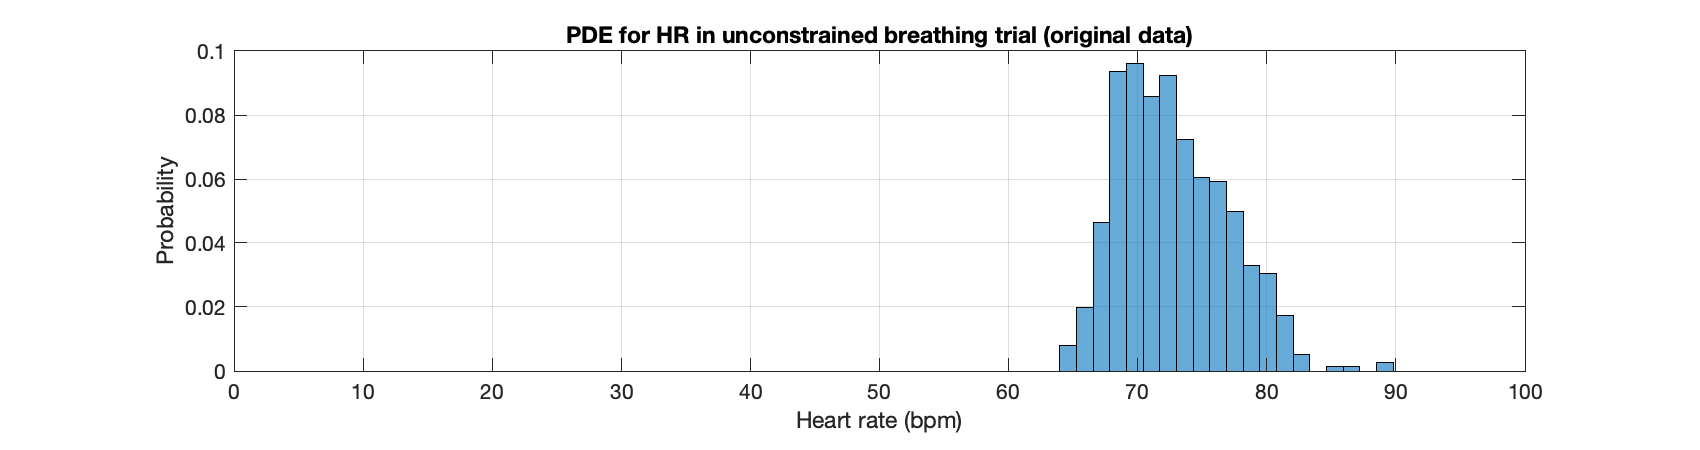
\includegraphics[width=\linewidth]{assignment2figs/pde_uncon.eps}
  \caption{Original data.}
  \label{fig:pde1}
\end{subfigure}\hfil 
\medskip
\begin{subfigure}{0.6\textwidth}
  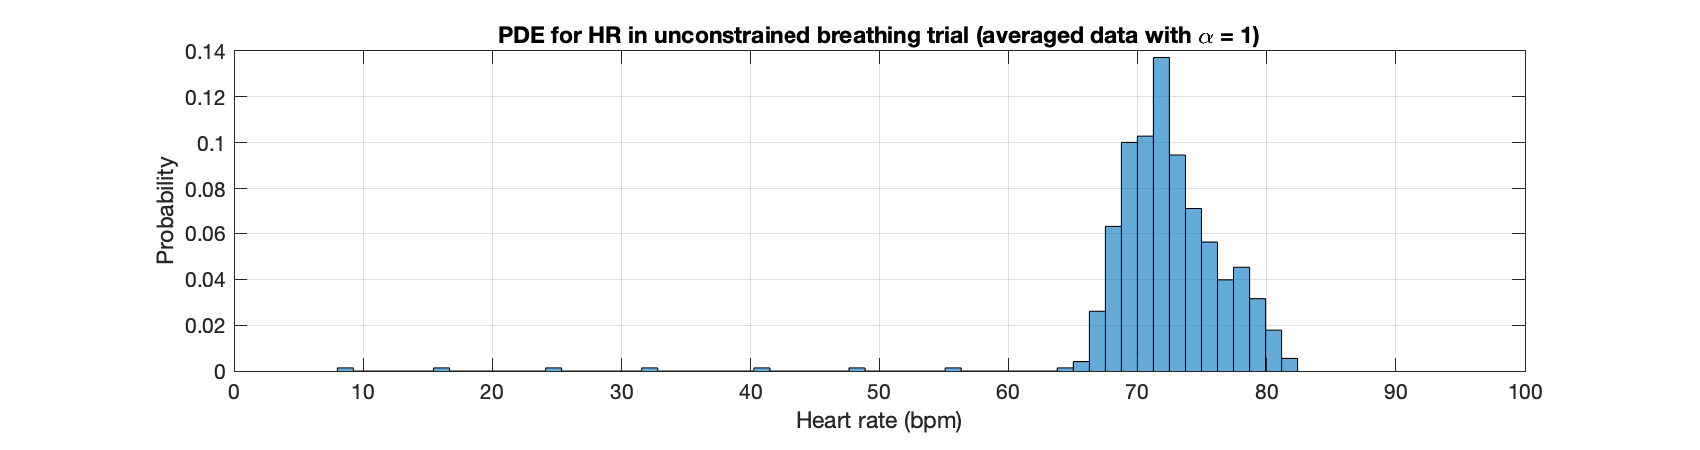
\includegraphics[width=\linewidth]{assignment2figs/pde_uncon1.eps}
  \caption{Data averaged using $\alpha = 1$.}
  \label{fig:pde2}
\end{subfigure}\hfil 
\medskip
\begin{subfigure}{0.6\textwidth}
  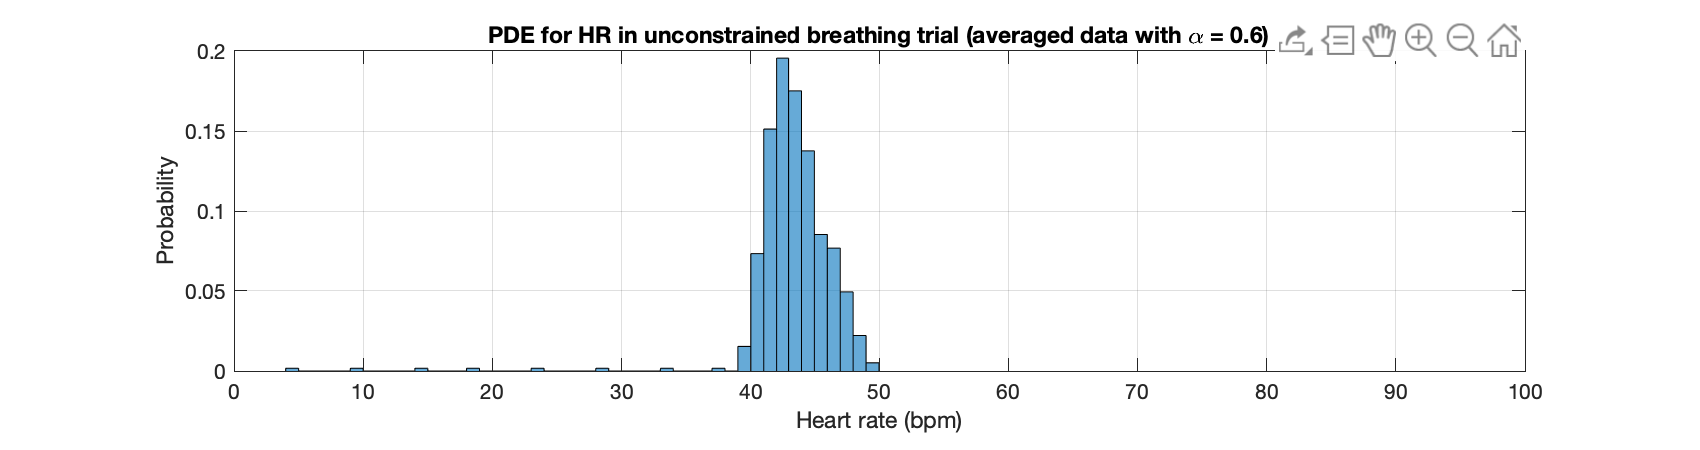
\includegraphics[width=\linewidth]{assignment2figs/pde_uncon06.eps}
  \caption{Data averaged using $\alpha = 0.6$.}
  \label{fig:pde3}
\end{subfigure}
\caption{PDEs for Trial 1 (unconstrained breathing).}
\label{fig:pdes}
\end{center}
\end{figure}

\noindent
The mean of the original signal is 72.8 and the SD is 4.24. From Figure \ref{fig:pdes}(\ref{fig:pde2}), averaging the signal appears to have a 'sharpening' effect on one side of the distribution, removing high frequency outliers whilst low frequency outliers remain. This is because averaging has a similar effect to a LPF of the data. The mean of the averaged distribution with $\alpha = 1$ is 72.2, whilst the variance ie 5.85. Whilst there is negligible impact on the mean, the low frequency harmonics that are included have the effect of increasing SD. Reducing $\alpha $ to 0.6, as in \ref{fig:pde3} reveals that $\alpha$ shifts the mean of the data from to 43.3 and the SD to 3.51. Such an effect on the mean is to be expected based on Equation \ref{eqn:pde}, since $\alpha$ acts as a scaling coefficient for all values. The reduction in SD can be explained by the 'sharpening' effect of low-pass filtering mentioned above.

\subsubsection{AR modelling of heart beat}

The ACFs for the RRI signals of each trial were calculated and are displayed in Figure \ref{fig:hr_acfs}.

\begin{figure}[H]
    \begin{center}
\begin{subfigure}{0.305\textwidth}
  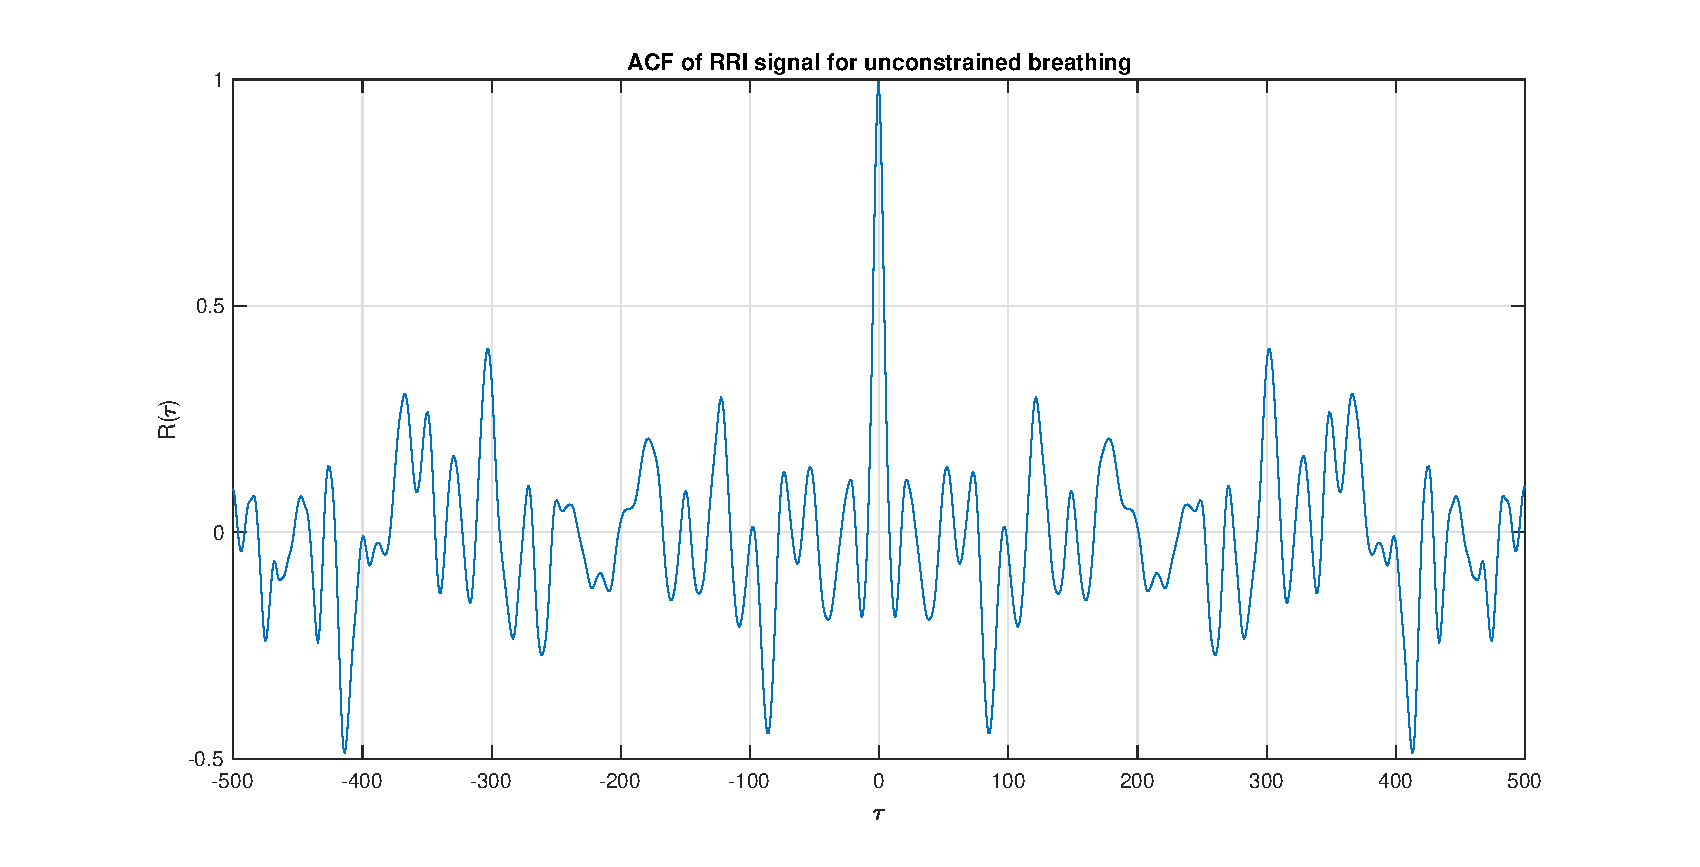
\includegraphics[width=\linewidth]{assignment2figs/acf_uncon.eps}
  \caption{ACF for Trial 1.}
  \label{fig:acft1}
\end{subfigure}
\begin{subfigure}{0.305\textwidth}
  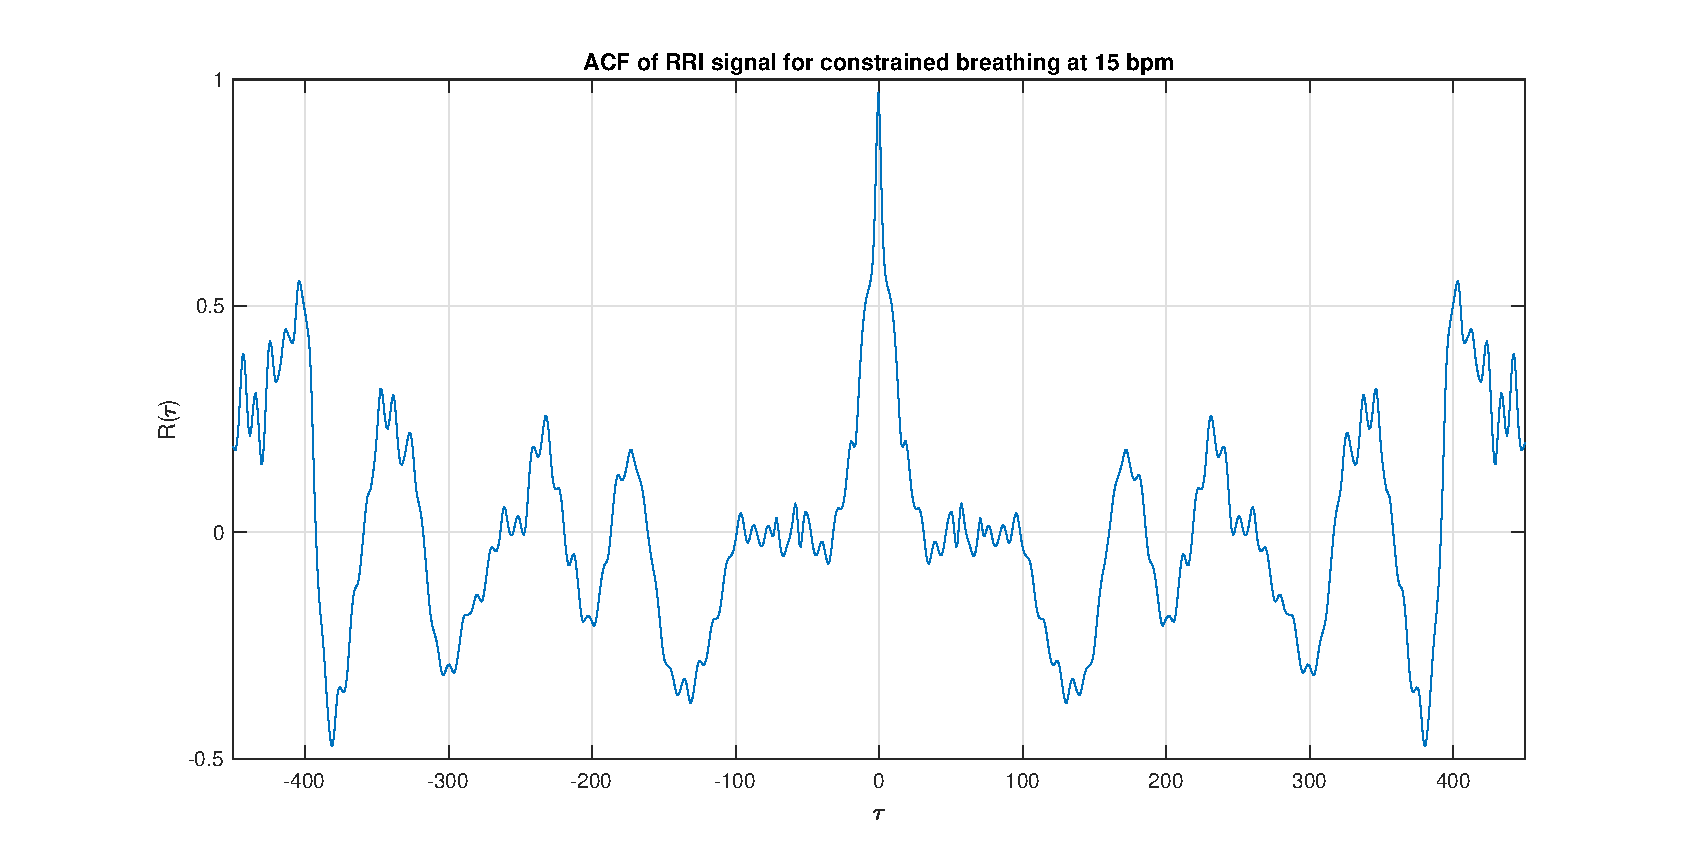
\includegraphics[width=\linewidth]{assignment2figs/acf_15.eps}
  \caption{ACF for Trial 2.}
  \label{fig:acft2}
\end{subfigure}
\begin{subfigure}{0.305\textwidth}
  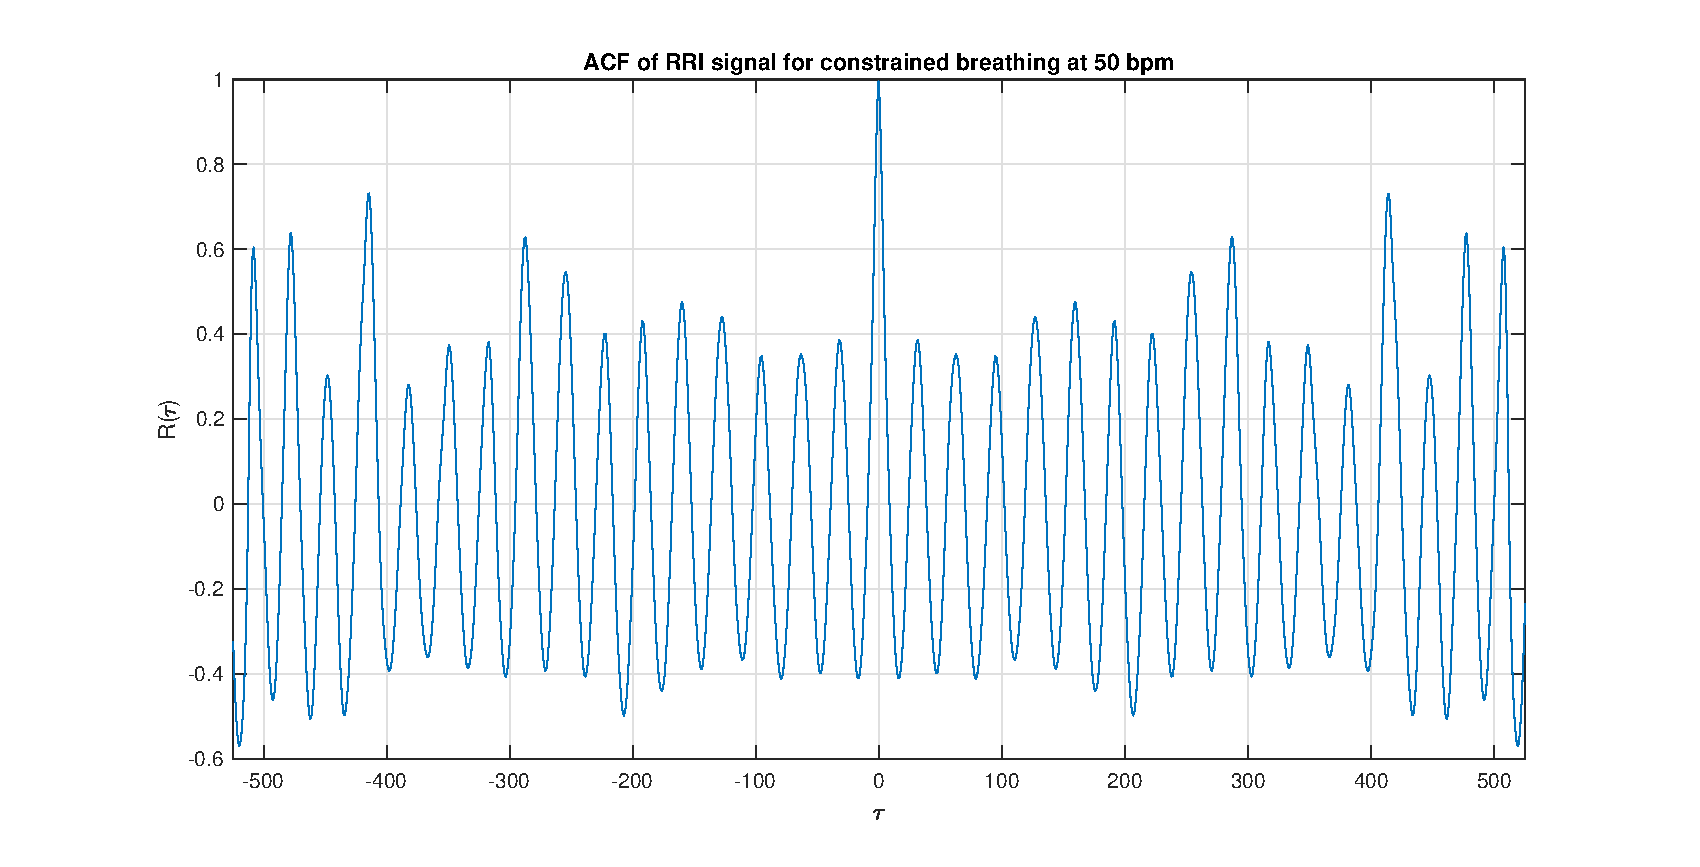
\includegraphics[width=\linewidth]{assignment2figs/acf_50.eps}
  \caption{ACF for Trial 3.}
  \label{fig:acft3}
\end{subfigure}
\caption{ACFs for Trial 1 (unconstrained breathing), 2 (constrained at 15 bpm) and 3 (constrained at 50 bpm).}
\label{fig:hr_acfs}
\end{center}
\end{figure}

\noindent
The ACFs for all trials are sinusiodal and of infinite length, suggesting that the RRI signal is an AR process. This implies that the current value of the signal has some dependence on previous values. To determine how many previous values this is (i.e. the model order), further investigation is required.

\vspace{0.5cm}
\noindent
In order to determine the correct model order, PACFs were  calculated for the RRI signals for each trial. These are shown in in Figure \ref{fig:HRstuff}.

\begin{figure}[H]
    \begin{center}
\begin{subfigure}{0.6\textwidth}
  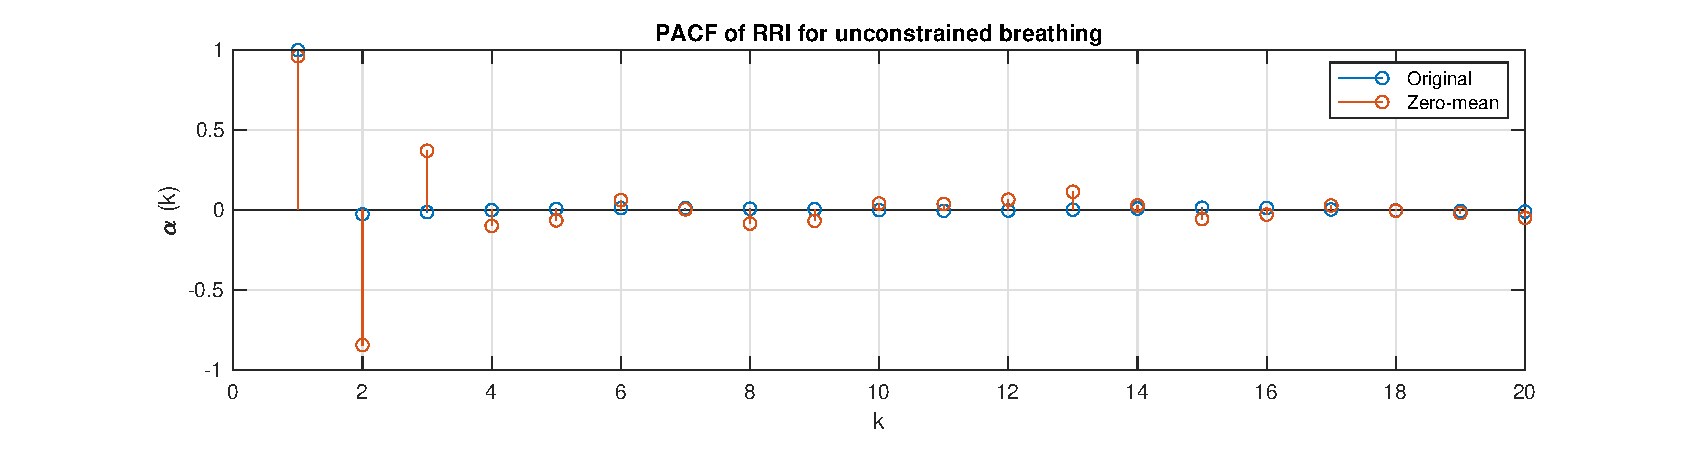
\includegraphics[width=\linewidth]{assignment2figs/pacf_uncon.eps}
  \caption{PACF for Trial 1.}
  \label{fig:pacfuncon}
\end{subfigure}\hfil 
\medskip
\begin{subfigure}{0.6\textwidth}
  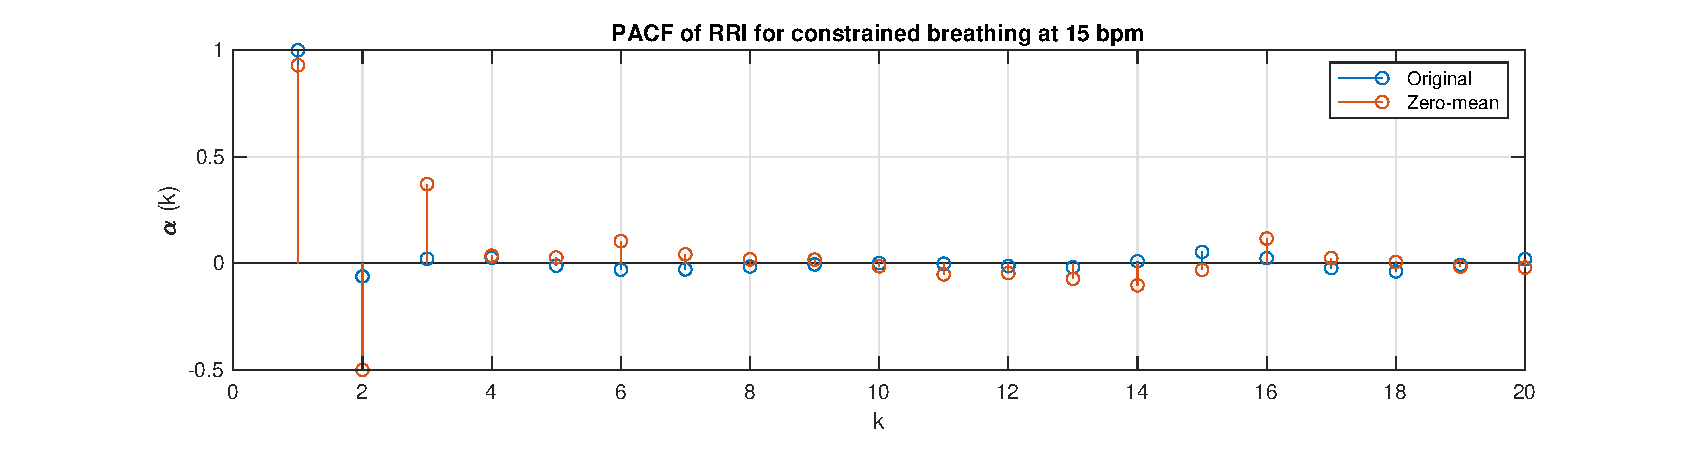
\includegraphics[width=\linewidth]{assignment2figs/pacf_15.eps}
  \caption{PACF for Trial 2.}
  \label{fig:pacf15}
\end{subfigure}\hfil 
\medskip
\begin{subfigure}{0.6\textwidth}
  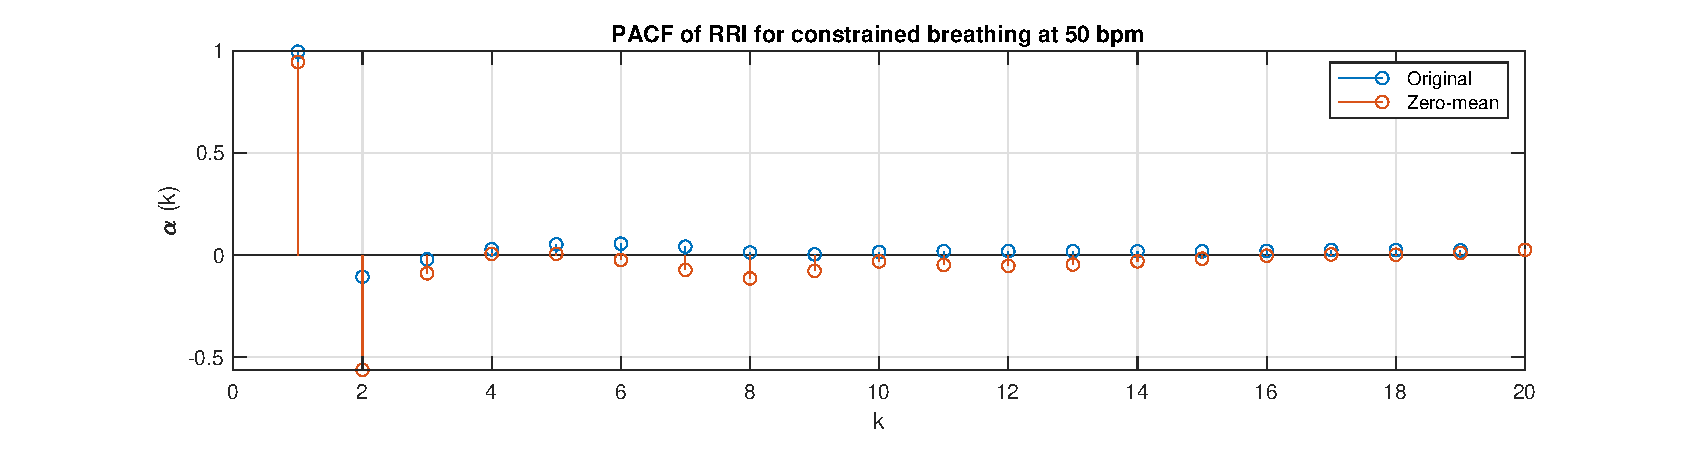
\includegraphics[width=\linewidth]{assignment2figs/pacf_50.eps}
  \caption{PACF for Trial 3.}
  \label{fig:pacf50}
\end{subfigure}
\caption{PACFs used to investigate AR model order for RRI signals.}
\label{fig:HRstuff}
\end{center}
\end{figure}

\noindent
The zero-mean PACF for Trial 1 in Figure \ref{fig:pacfuncon} appears to converge to zero for shifts above 2 or 3, implying that the correct model order is 2 or 3. The same is true for Trial 2 in Figure \ref{fig:pacf15}. However, the PACF of Trial 3 in Figure \ref{fig:pacf50} clearly converges to zero after shifts of 2, implying that the correct model order is 2. In order to confirm this, further statistical analysis is required.

\vspace{0.5cm}
\noindent
As in the previous section, the $MDL$, $AIC$ and $AIC_{C}$ can be used to determine the correct model order and resolve the uncertainty of the PACF-based estimate.

\begin{figure}[H]
    \begin{center}
\begin{subfigure}{0.31\textwidth}
  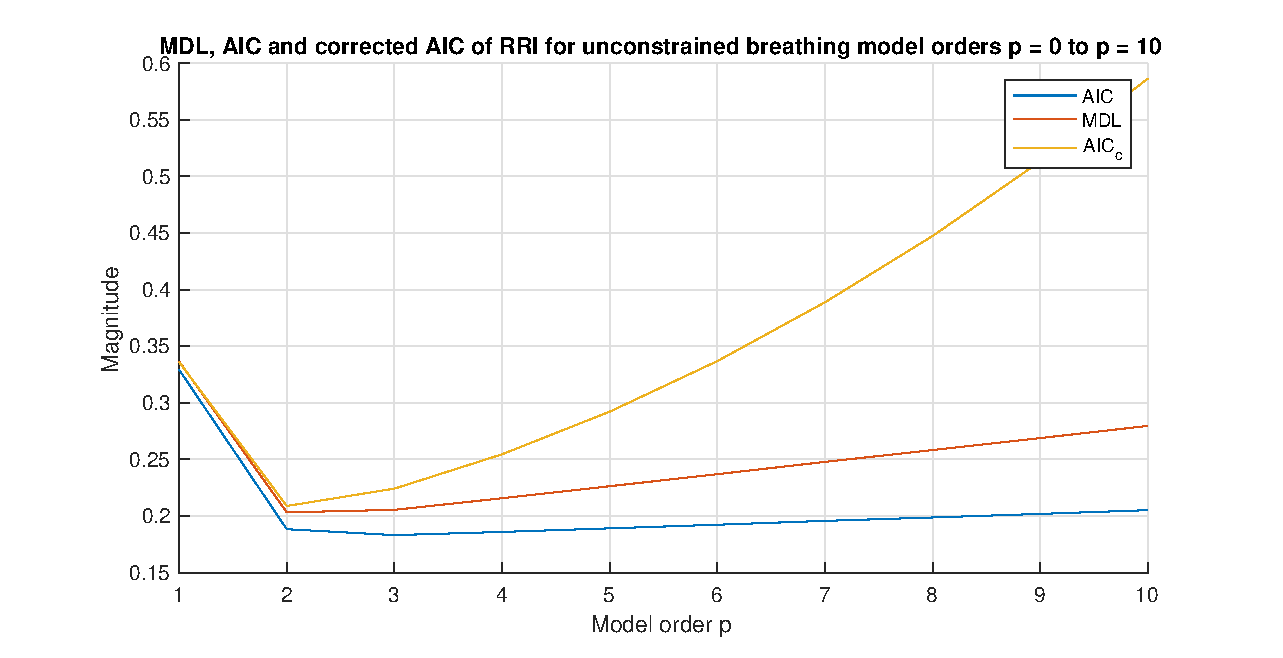
\includegraphics[width=\linewidth]{assignment2figs/mdl_aic_uncon.eps}
  \caption{$MDL$, $AIC$ and $AIC_{C}$ for Trial 1.}
\label{fig:1}
\end{subfigure}
\begin{subfigure}{0.31\textwidth}
  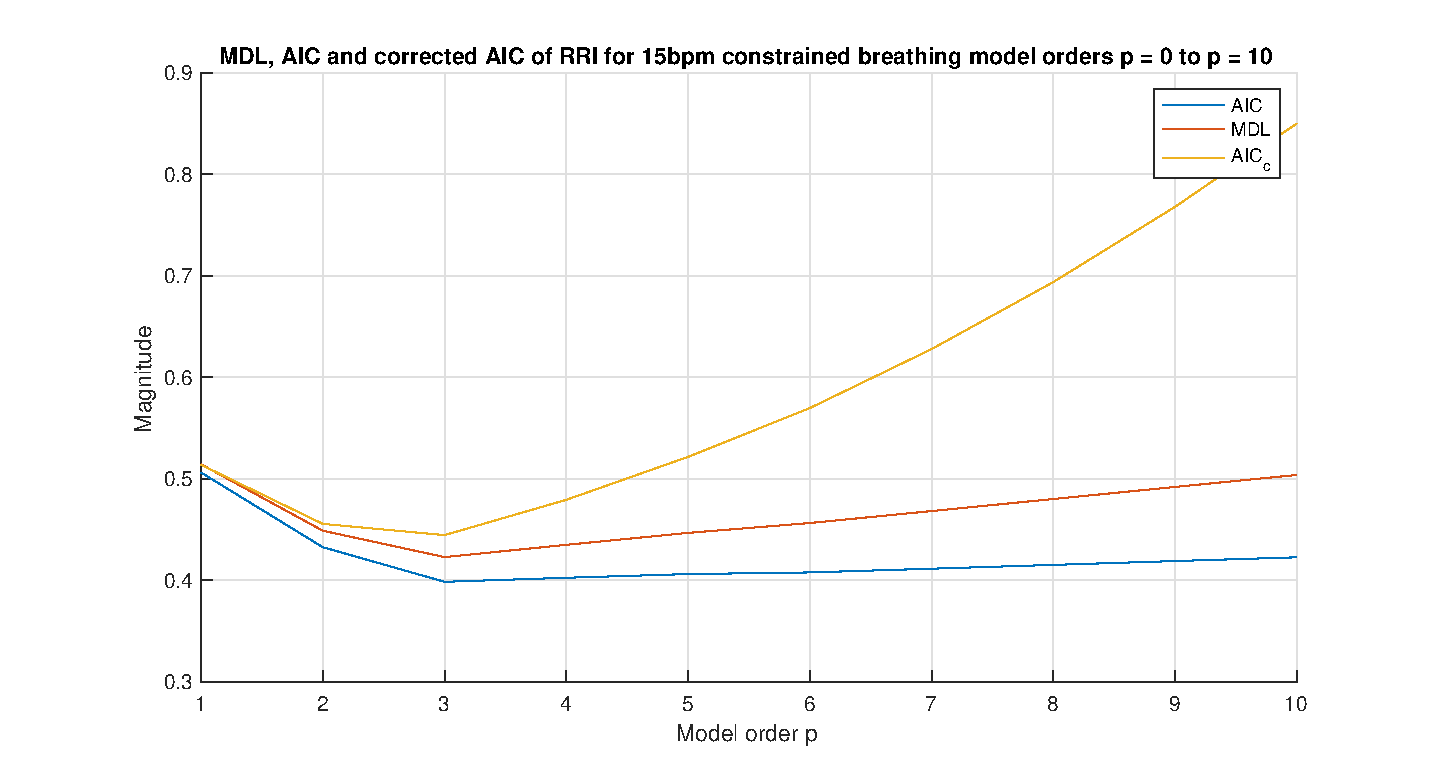
\includegraphics[width=\linewidth]{assignment2figs/mdl_aic_15.eps}
  \caption{$MDL$, $AIC$ and $AIC_{C}$ for Trial 2.}
  \label{fig:2}
\end{subfigure}
\begin{subfigure}{0.31\textwidth}
  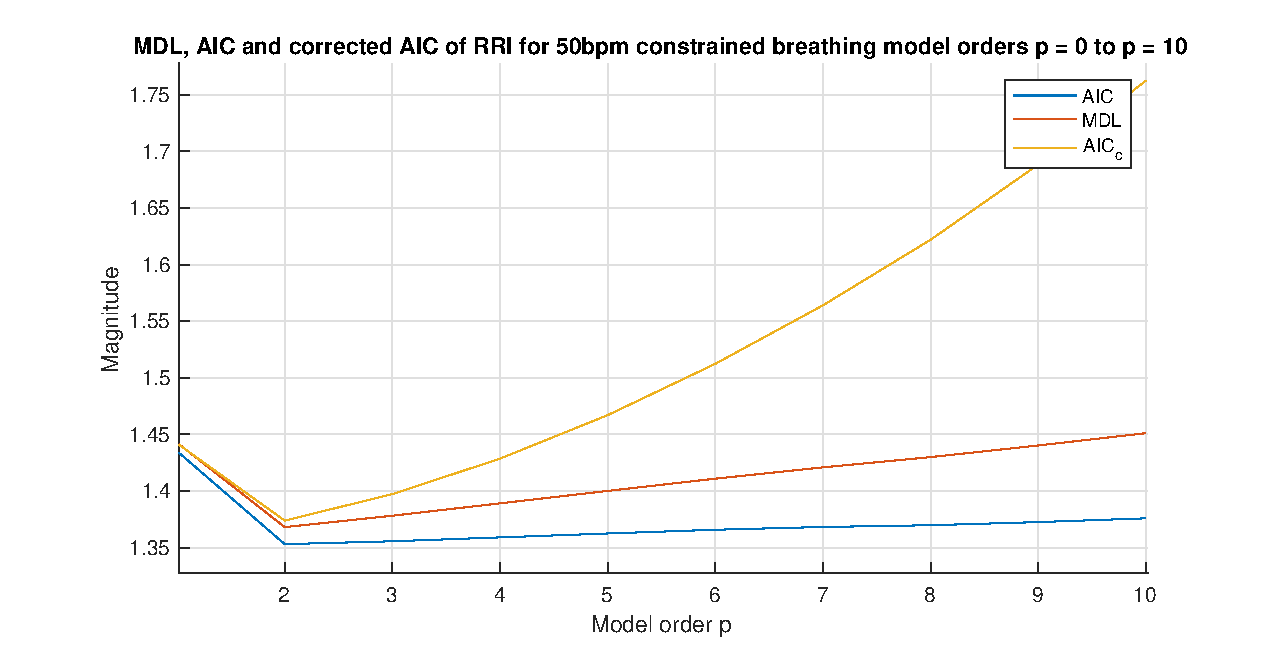
\includegraphics[width=\linewidth]{assignment2figs/mdl_aic_50.eps}
  \caption{$MDL$, $AIC$ and $AIC_{C}$ for Trial 3.}
    \label{fig:3}
\end{subfigure}
\caption{Statistical measures to investigate AR model order for RRI signals.}
\label{fig:HRmorestuff}
\end{center}
\end{figure}

\noindent
For Trial 1 in Figure \ref{fig:1}, the AIC global minimum is at 3 but the MDL global minimum is at 2, reflecting the uncertainty in model order from the PACFs. However, the corrected AIC global minimum is at 2, implying that Trial 1 can be modelled as an AR(2) process. For Trial 2 in Figure \ref{fig:2}, the global minima for all measures are at 3, agreeing with what was seen in the PACFs and implying that Trial 2 can be modelled as an AR(3) process. Finally, for Trial 3 in Figure \ref{fig:3}, the global minima for all measures are at 2, again agreeing with what was seen in the PACFs and implying that Trial 3 can be modelled as an AR(2) process.